% !TeX root = ../../Skript.tex
\cohead{\Large\textbf{Grafisches Ableiten}}
\fakesubsection{Grafisches Ableiten}
Die Geschwindigkeit ist ein weiteres Beispiel für eine Änderungsrate. Sie gibt an wie stark sich der Ort mit der Zeit verändert. Betrachten wir einen Ausschnitt einer Fahrt auf der Autobahn:

\smallskip

\begin{minipage}[t]{\textwidth}
	\centering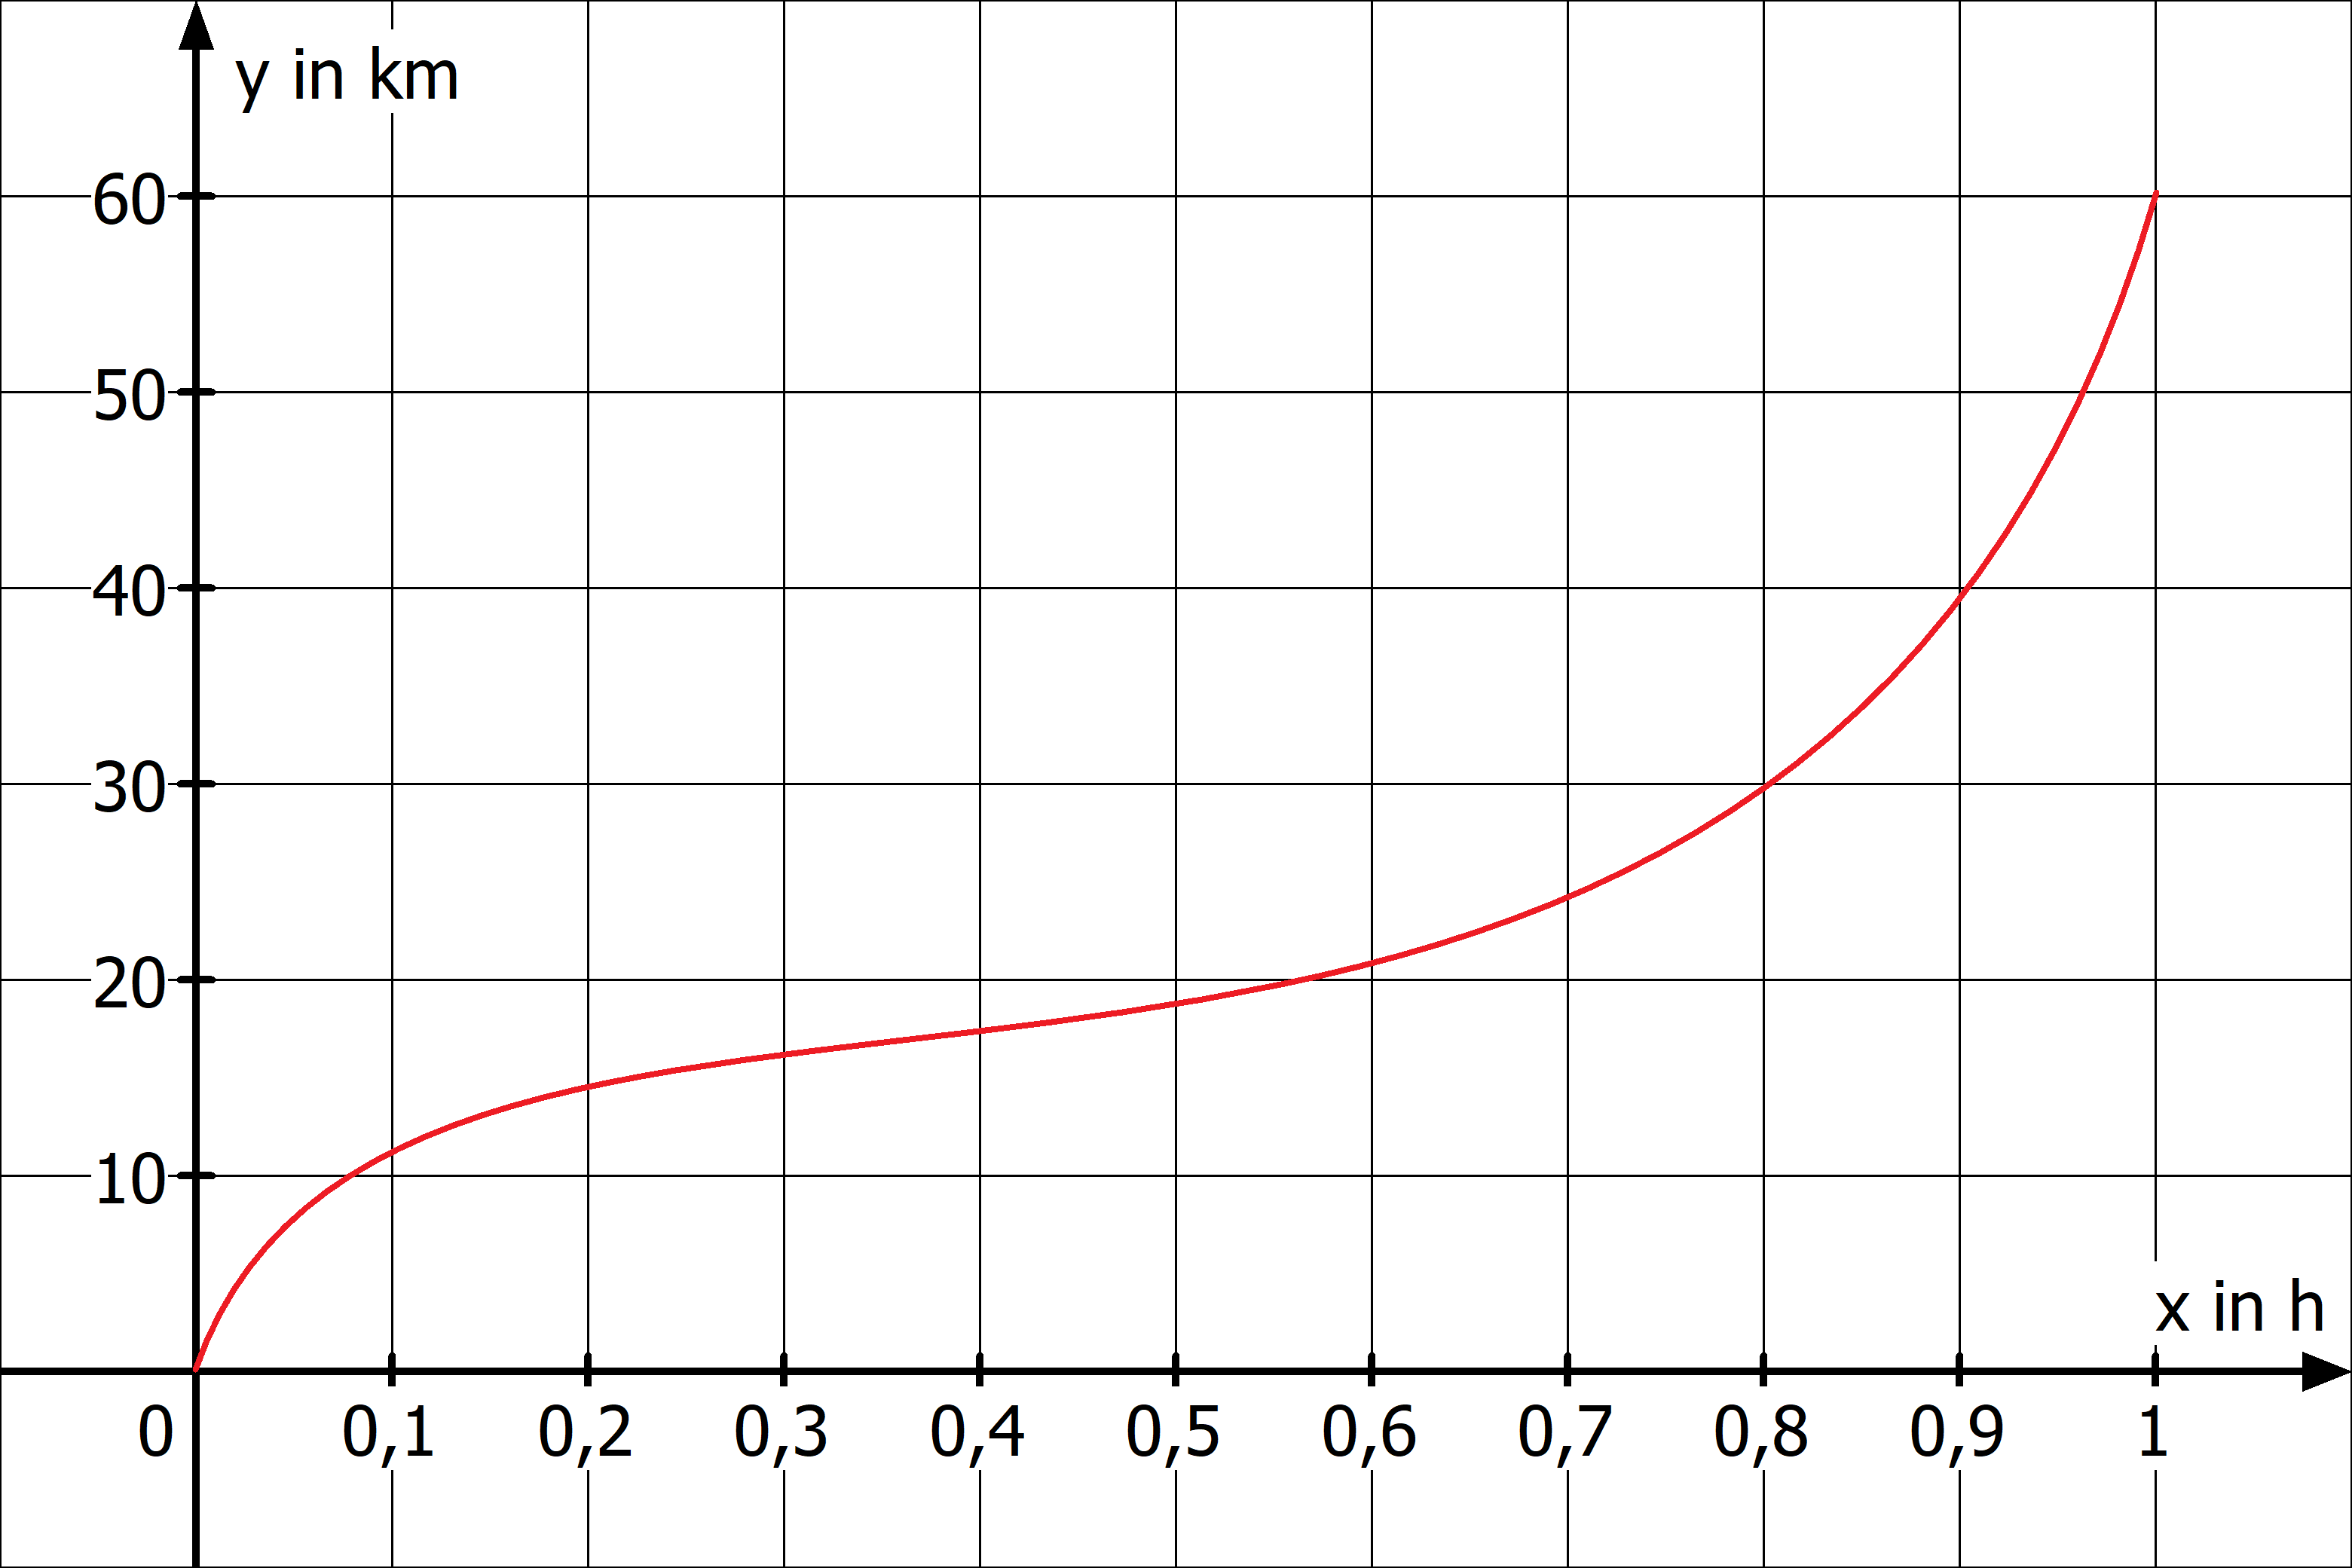
\includegraphics[width=\textwidth]{\ableitung/pics/momentan_Geschwindigkeit.png}
\end{minipage}

Im obigen Beispiel lässt sich die Durchschnittsgeschwindigkeit in der ersten Stunde wie folgt berechnen: \(\frac{60km-0km}{1h-0h}=60\frac{km}{h}\). Man kann leicht erkennen, dass die momentane Geschwindigkeit (auf dem Tacho angezeigte Geschwindigkeit) nicht gleich bleibt, da die Kurve sonst eine Gerade sein müsste. Doch wie kann man die momentane Geschwindigkeit z.B. nach \(0,3h\) bestimmen?

Rein vom Verlauf der Kurve her, muss die Geschwindigkeit kleiner als \(60\frac{km}{h}\) sein, da die Kurve bei \(0,3h\) relativ flach verläuft. Eine bessere Schätzung würde man erhalten, indem man die Durchschnittsgeschwindigkeit von \(0,3h\) bis \(1h\) bestimmt: \(\frac{60km-17km}{1h-0,3h}\approx61\frac{km}{h}\). Das Auto hatte in den letzten 42 Minuten also eine durchschnittliche Geschwindigkeit von \(61\frac{km}{h}\), was eine sogar noch schlechtere Schätzung ist.

Etwas besser wäre es, die rechte Grenze etwas weiter nach links zu schieben, also nicht den Zeitraum von \(0,3h\) bis \(1h\) zu betrachten, sondern von \(0,3h\) bis \(0,6h\): \(\frac{21km-17km}{0,6h-0,3h}\approx13\frac{km}{h}\). Diese Schätzung scheint schon deutlich besser zu sein.

Letztlich bestimmen wir die Steigung einer Geraden mit Hilfe eines Steigungsdreiecks, wobei 2 Ecken des Dreiecks auf dem Schaubild der Funktion liegen. Je näher wir die beiden Ecken zusammenschieben, desto näher liegt das Ergebnis an der momentanen Änderungsrate. Mathematisch kann man die 2 Ecken auf einen Punkt zusammenschieben, um die tatsächliche momentane Änderungsrate zu bestimmen. Grafisch wird aus der Geraden dann eine Tangente (vergleiche Tangenten bei der gegenseitigen Lage von Geraden und Parabel). Im obigen Beispiel hätte die Tangente an der Stelle \(0,3h\) eine Steigung von ca. \(12\frac{km}{h}\), was der auf dem Tacho angezeigten Geschwindigkeit entsprechen würde.\newpage
\begin{tcolorbox}

    \bigskip

	\textcolor{loestc}{Die momentane Änderungsrate bzw. Ableitung einer Funktion an einer Stelle \(x_0\) entspricht der Steigung der Tangenten an dieser Stelle. Die Begriffe momentane Änderungsrate, Ableitung und Steigung (kurz für Tangentensteigung) werden meist synonym verwendet.}

    \bigskip

\end{tcolorbox}
\begin{minipage}{\textwidth}
	\adjustbox{valign=t, padding=0ex 0ex 2ex 0ex}{\begin{minipage}{0.5\textwidth-2ex}
		\centering\includegraphics[width=\textwidth]{\ableitung/pics/0komma5xquadrat\iftoggle{ausfuellen}{}{_empty}.png}
	\end{minipage}}%
	\adjustbox{valign=t, padding=2ex 0ex 0ex 0ex}{\begin{minipage}{0.5\textwidth-2ex}
		Wert der Ableitung von \(f(x)=0,5x^2\) grafisch bestimmt:

		An der Stelle \(x_0=1\): Die Tangente an der Stelle \(x=1\) hat eine Steigung von ca. 1, also beträgt die Ableitung 1.

		An der Stelle \(x_1=2\): \textcolor{loes}{Die Tangente an der Stelle \(x=2\) hat eine Steigung von ca. 2, also beträgt die Ableitung 2.}

		An der Stelle \(x_2=0\): \textcolor{loes}{Die Tangente an der Stelle \(x=0\) hat eine Steigung von 0, also beträgt die Ableitung 0.}

		An der Stelle \(x_0=-3\): \textcolor{loes}{Die Tangente an der Stelle \(x=-3\) hat eine Steigung von ca. -3, also beträgt die Ableitung -3.}

	\end{minipage}}%
\end{minipage}
\begin{tcolorbox}

    \bigskip

	\textcolor{loestc}{Wir führen als Symbol für die Ableitung \(f'(x)\), sprich f Strich von x, ein.}

	\textcolor{loestc}{\(f'(1)=2\) (sprich f Strich von 1 gleich 2) bedeutet also, dass die Ableitung von f an der Stelle 1 gleich 2 beträgt. Würde man die Tangente an \(f\) an der Stelle 1 zeichnen, so hätte sie eine Steigung von 2.}

    \bigskip

\end{tcolorbox}
Zusammengefassung: Die momentane Änderungsrate/Ableitung/Steigung einer Funktion gibt also an, wie stark sich die Funktion an einer Stelle ändert (statt innerhalb eines Intervalls wie bei der durchschnittlichen Änderungsrate). Steigt die Funktion, ist die Ableitung positiv, fällt die Funktion ist sie negativ. Je steiler das Schaubild nach oben geht, desto größer ist die Steigung und damit auch die Ableitung. Grafisch lässt sich die Ableitung mit Hilfe der Tangentensteigung abschätzen.
\newpage
%%%%%%%%%%%%%%%%%%%%%%%%%%%%%%%%%%%%%%%%%%%%%%%%%%%%%%%%%%%%%%%%%%%%%%%%%%%%%%%%%%%%%%%%%%%%%%%%%%%%%%
\begin{Exercise}[title={\raggedright Schätze jeweils die Ableitung an den Stellen -2, 0, 1 und 3 ab.}, label=grafischABlA1]

    \begin{minipage}{\textwidth}
		\begin{minipage}{\textwidth}
			\begin{minipage}{0.5\textwidth}
				\centering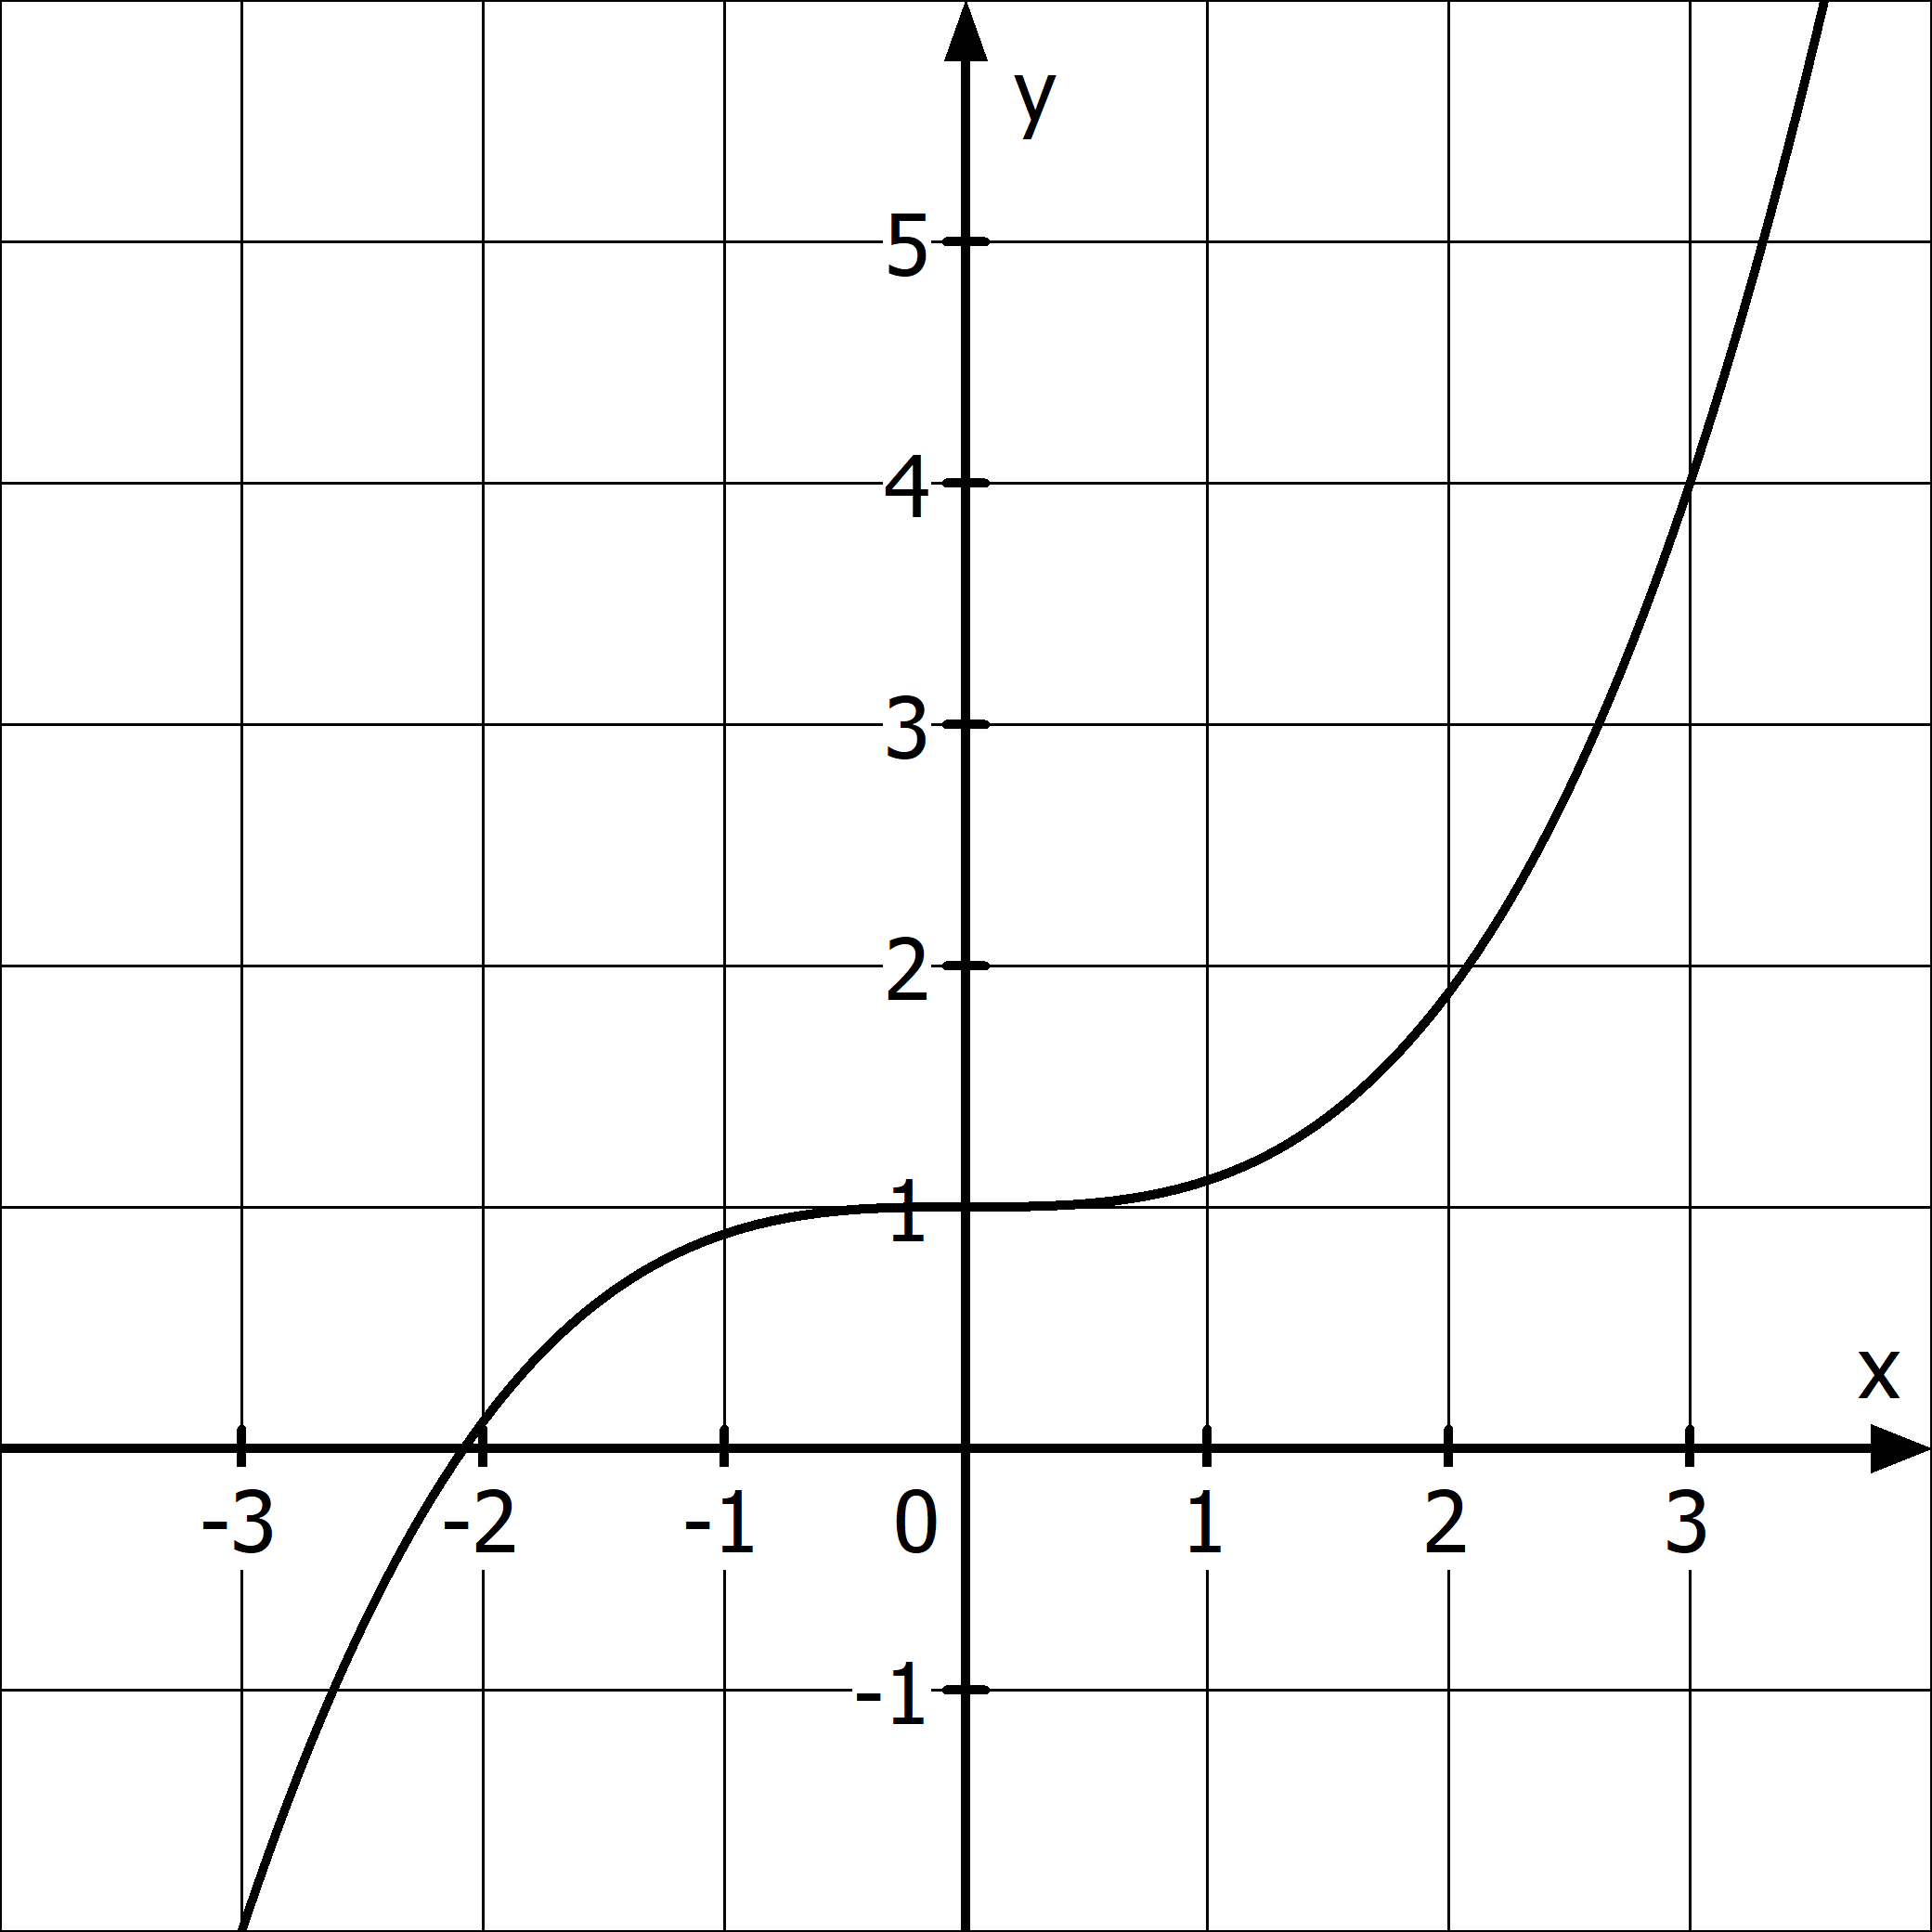
\includegraphics[width=.95\textwidth]{\ableitung/pics/grafisch1.png}
			\end{minipage}%
			\begin{minipage}{0.5\textwidth}
				\centering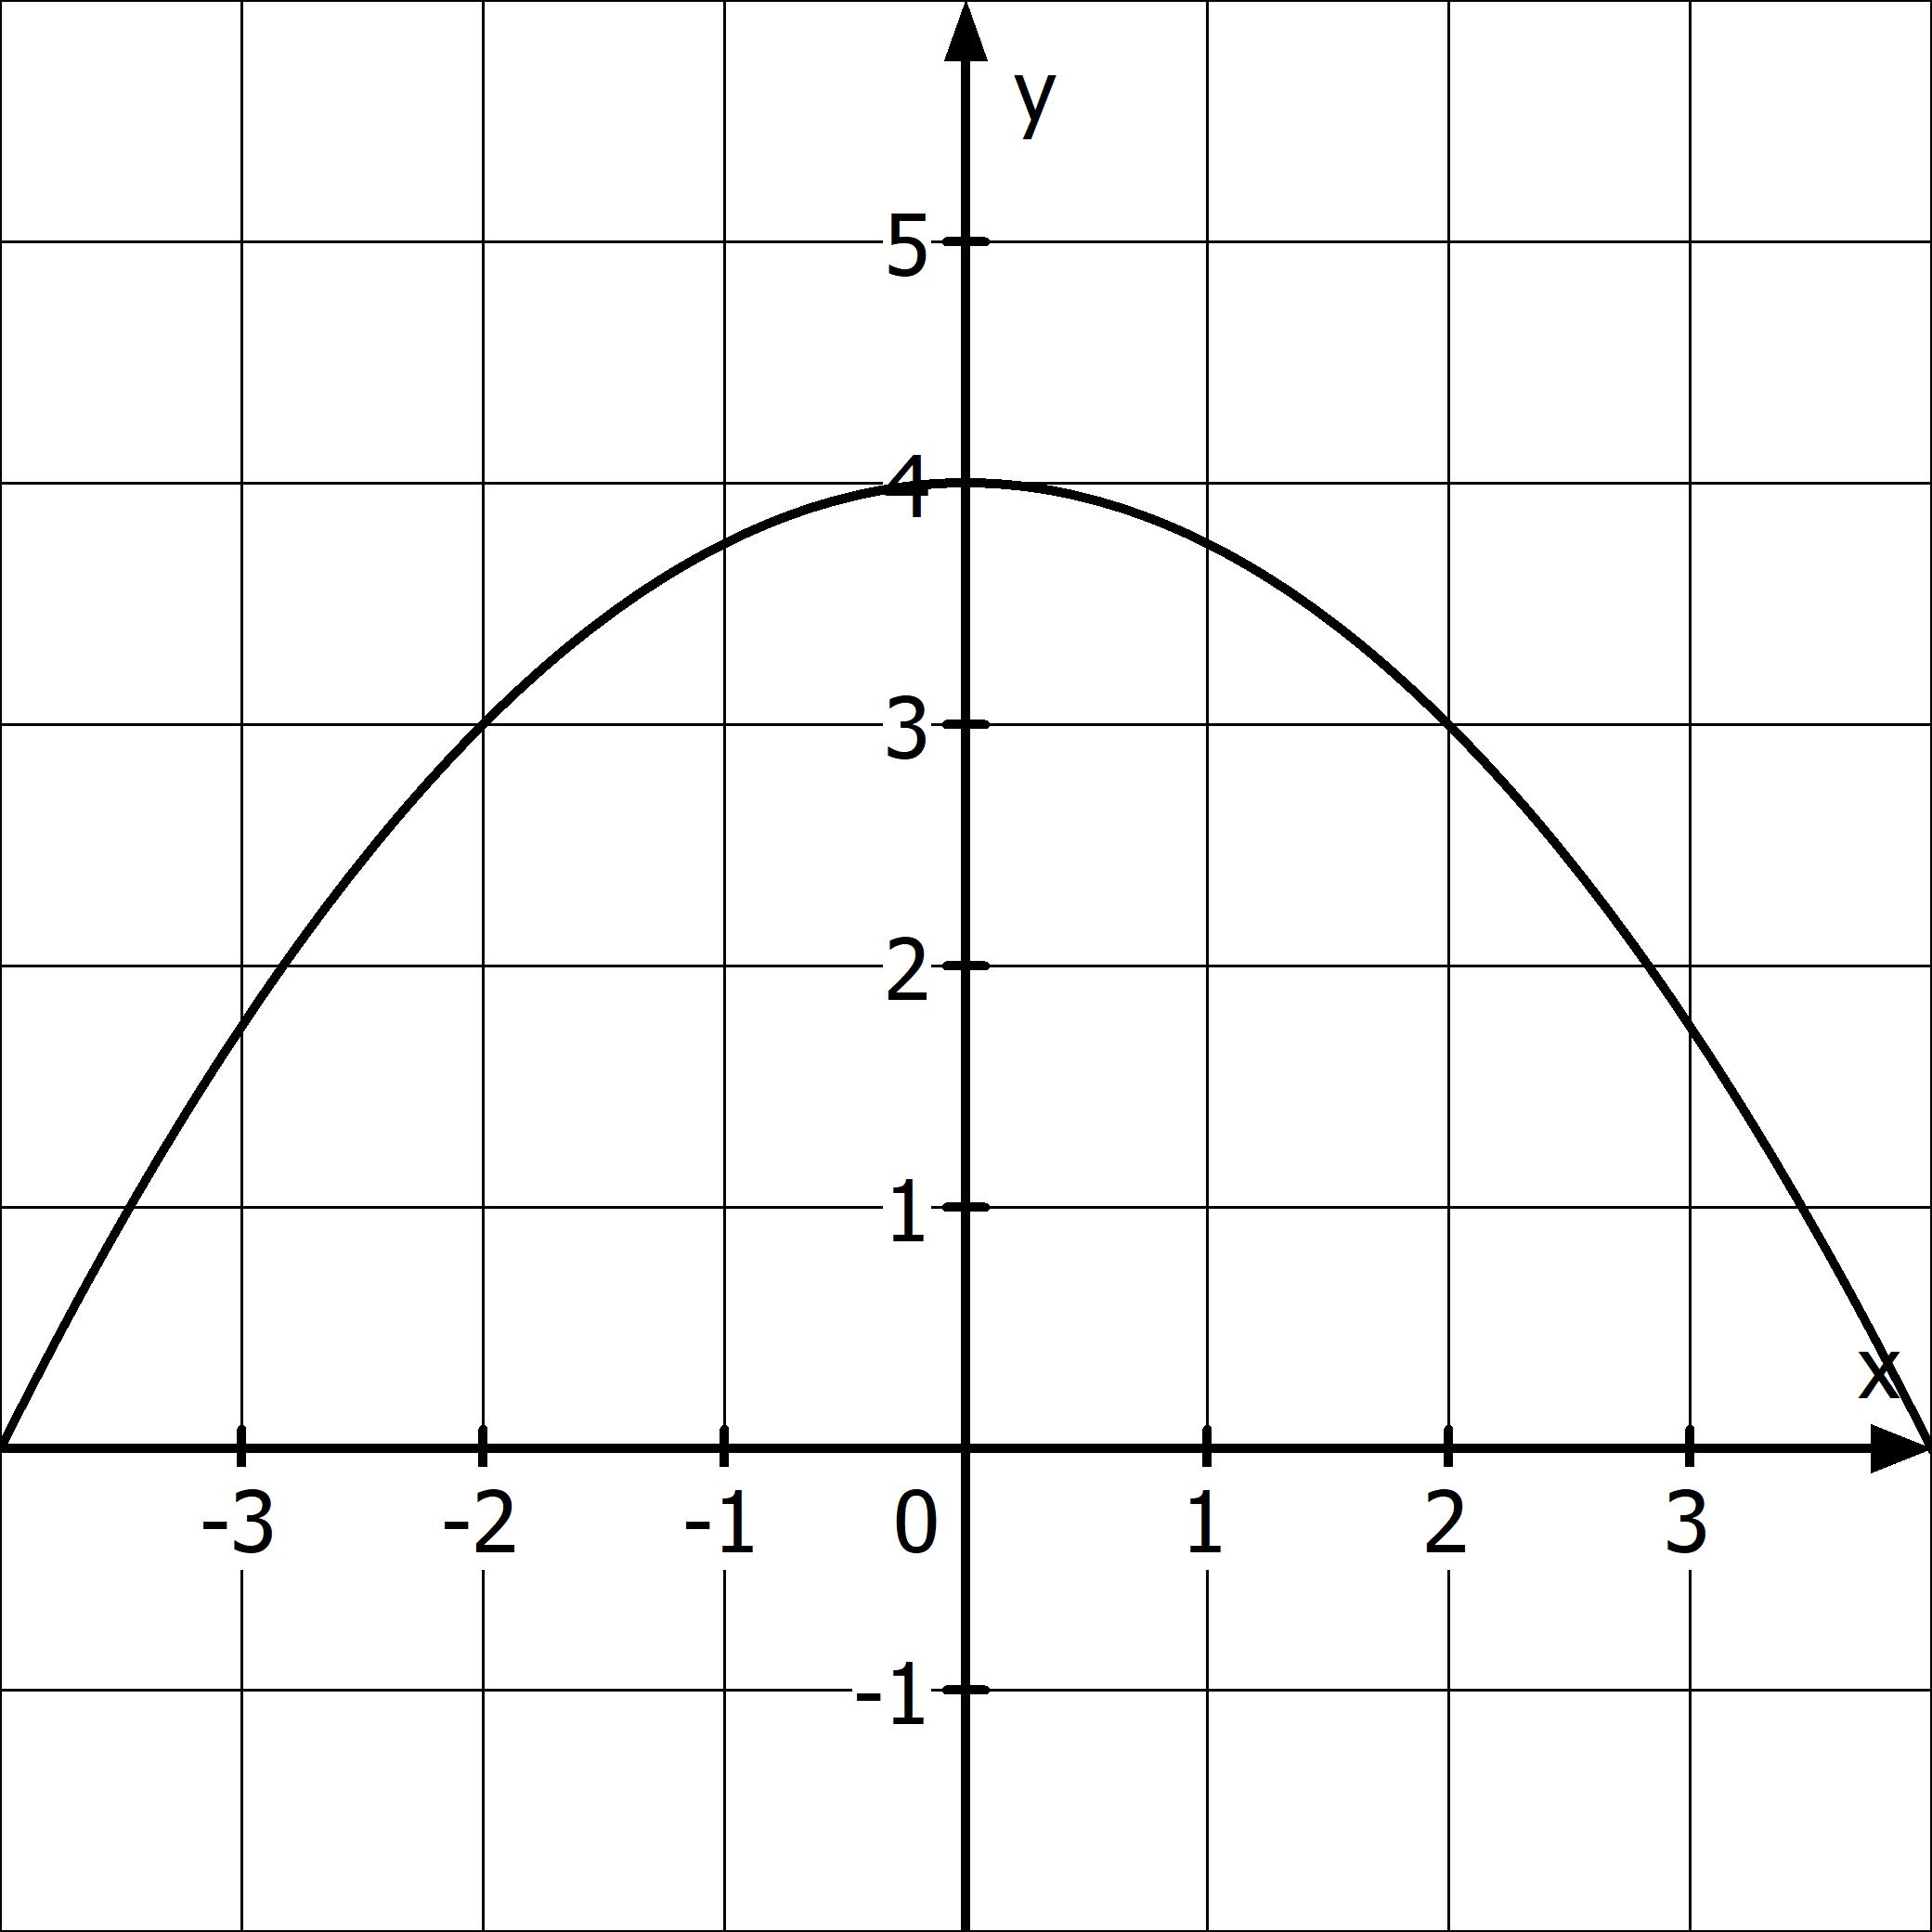
\includegraphics[width=.95\textwidth]{\ableitung/pics/grafisch2.png}
			\end{minipage}%
		\end{minipage}%

        \bigskip

		\begin{minipage}{\textwidth}
			\begin{minipage}{0.5\textwidth}
				\centering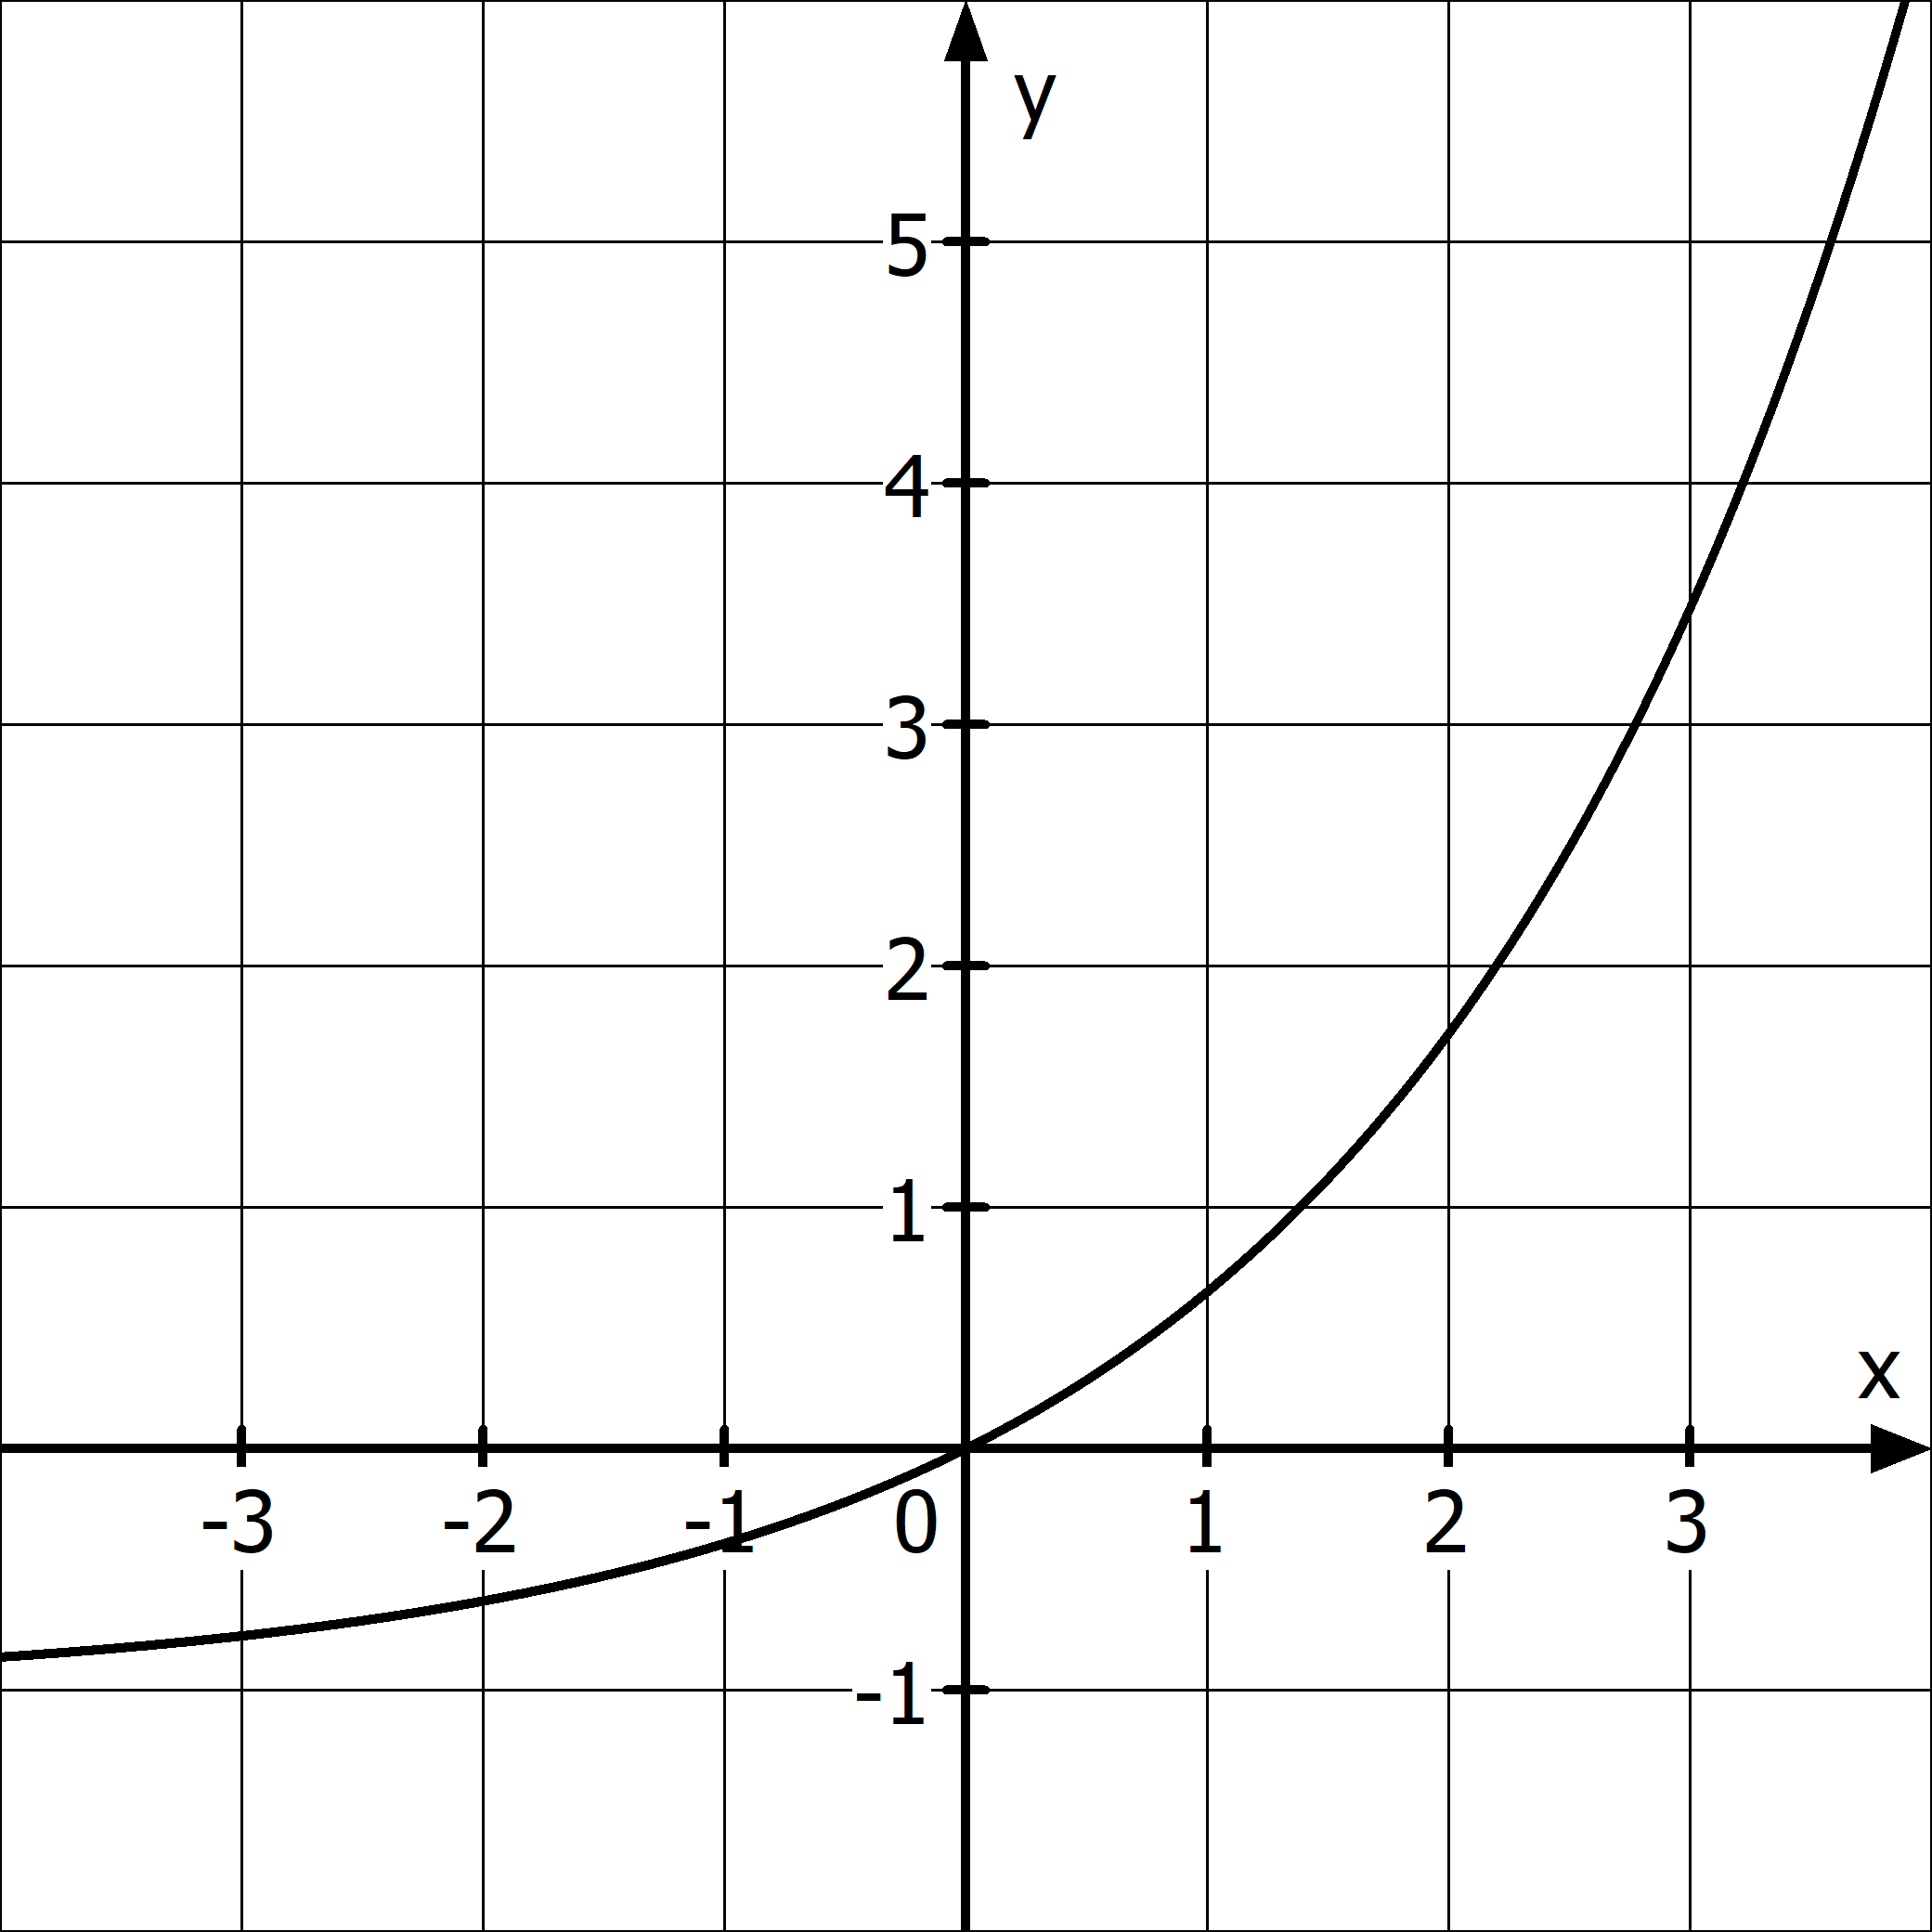
\includegraphics[width=.95\textwidth]{\ableitung/pics/grafisch3.png}
			\end{minipage}%
			\begin{minipage}{0.5\textwidth}
				\centering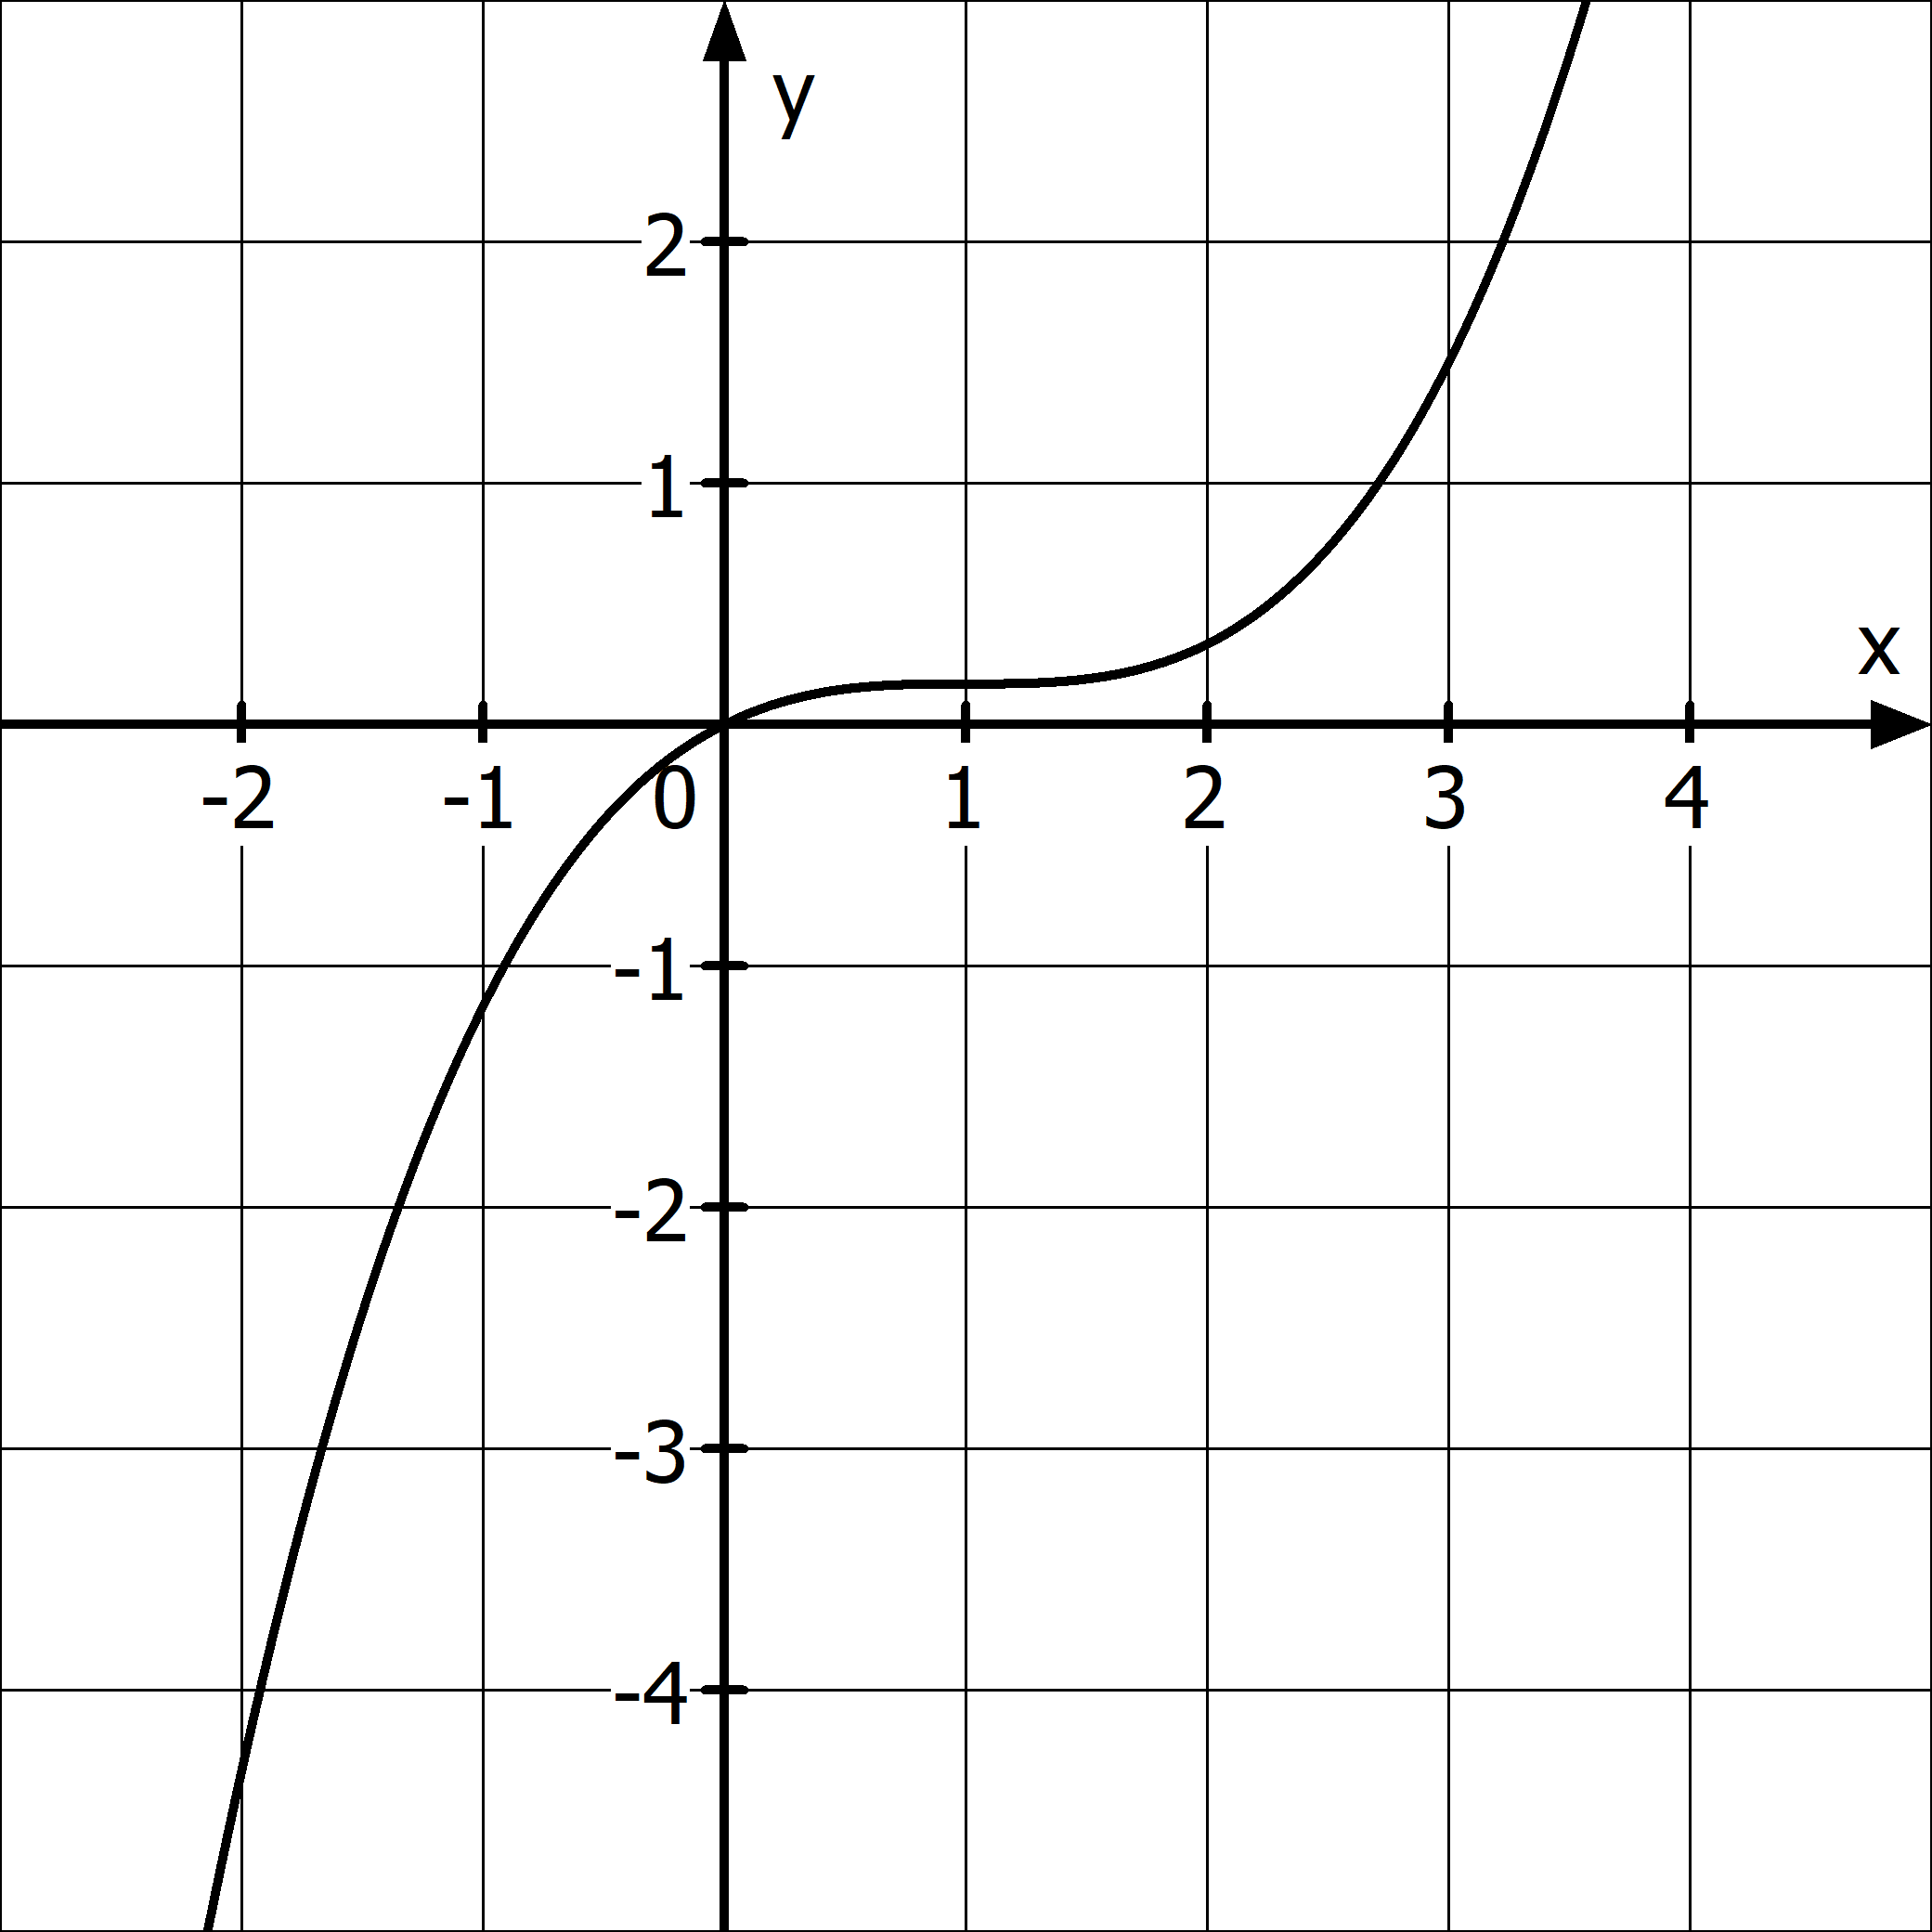
\includegraphics[width=.95\textwidth]{\ableitung/pics/grafisch4.png}
			\end{minipage}%
		\end{minipage}%
    \end{minipage}
\end{Exercise}
%%%%%%%%%%%%%%%%%%%%%%%%%%%%%%%%%%%%%%%%%
\begin{Answer}[ref=grafischABlA1]\\
	\begin{minipage}{\textwidth}
		\begin{minipage}{0.5\textwidth}
			\centering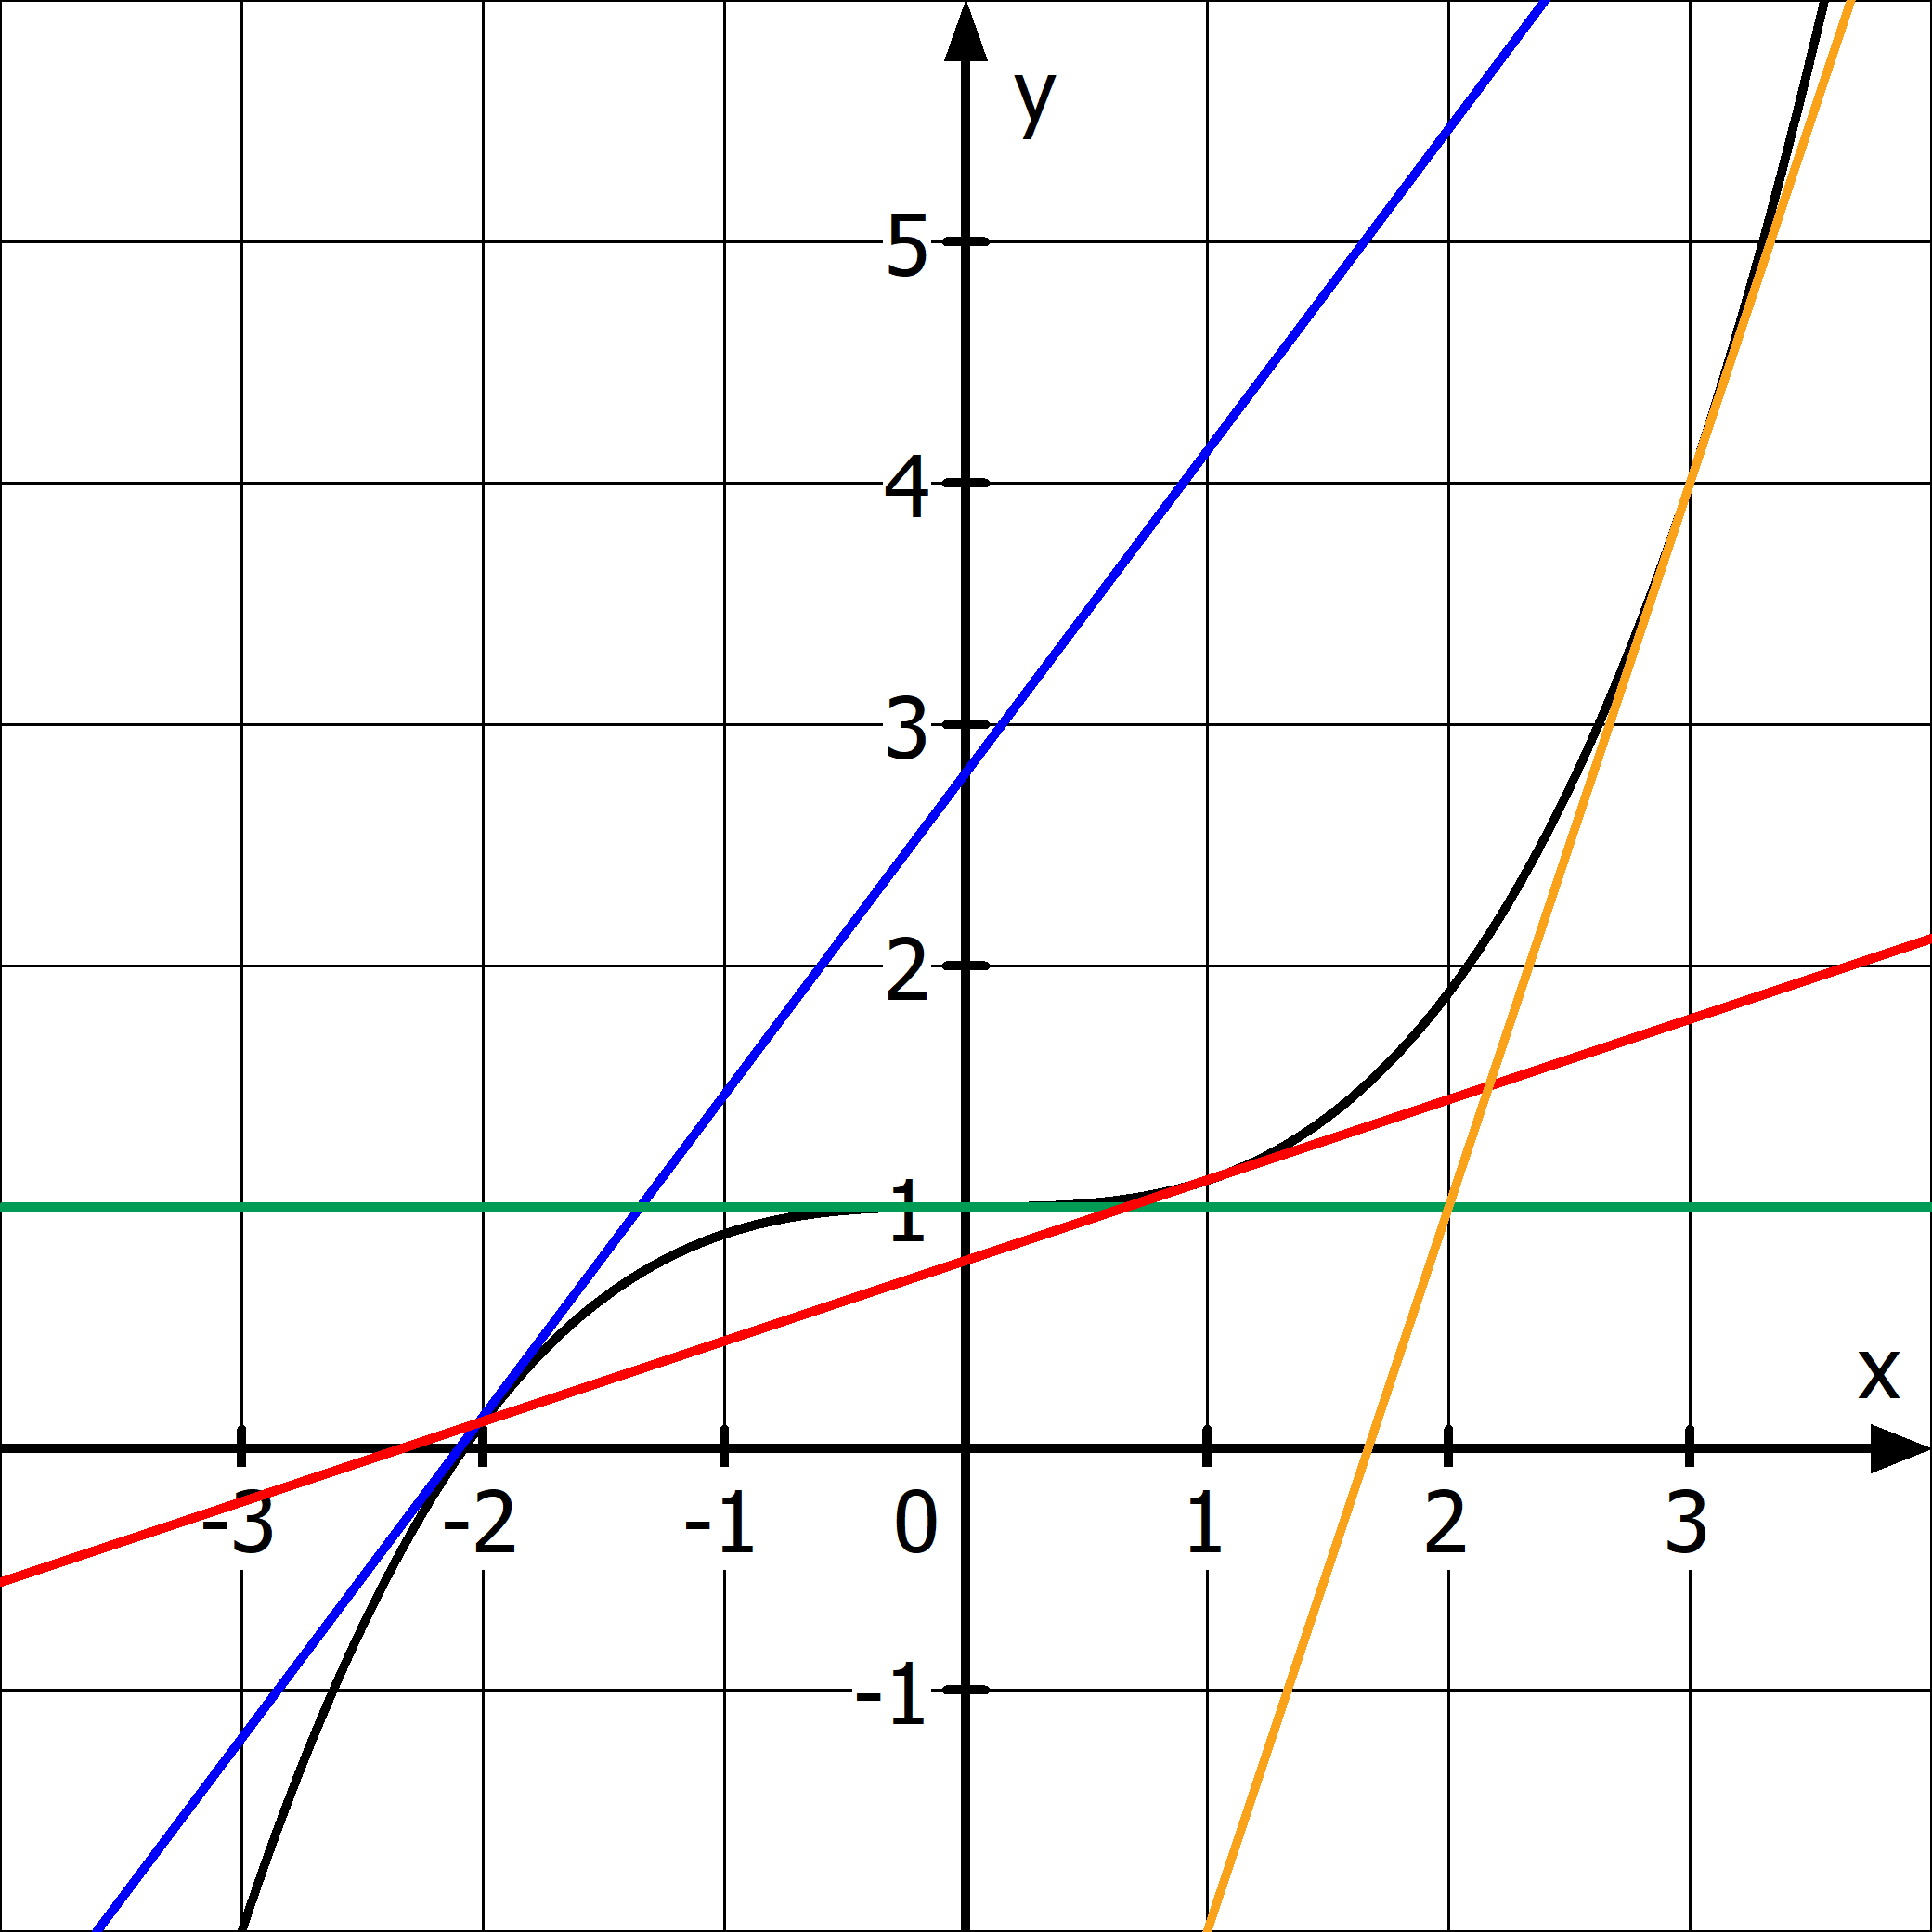
\includegraphics[width=.95\textwidth]{\ableitung/pics/grafisch1Loesung.png}\\
			\(\textcolor{blue}{f'(-2)\approx\frac{4}{3}}\)\\
			\(\textcolor{ForestGreen}{f'(0)\approx0}\)\\
			\(\textcolor{red}{f'(1)\approx\frac{1}{3}}\)\\
			\(\textcolor{YellowOrange}{f'(3)\approx 3}\)\\
		\end{minipage}%
		\begin{minipage}{0.5\textwidth}
			\centering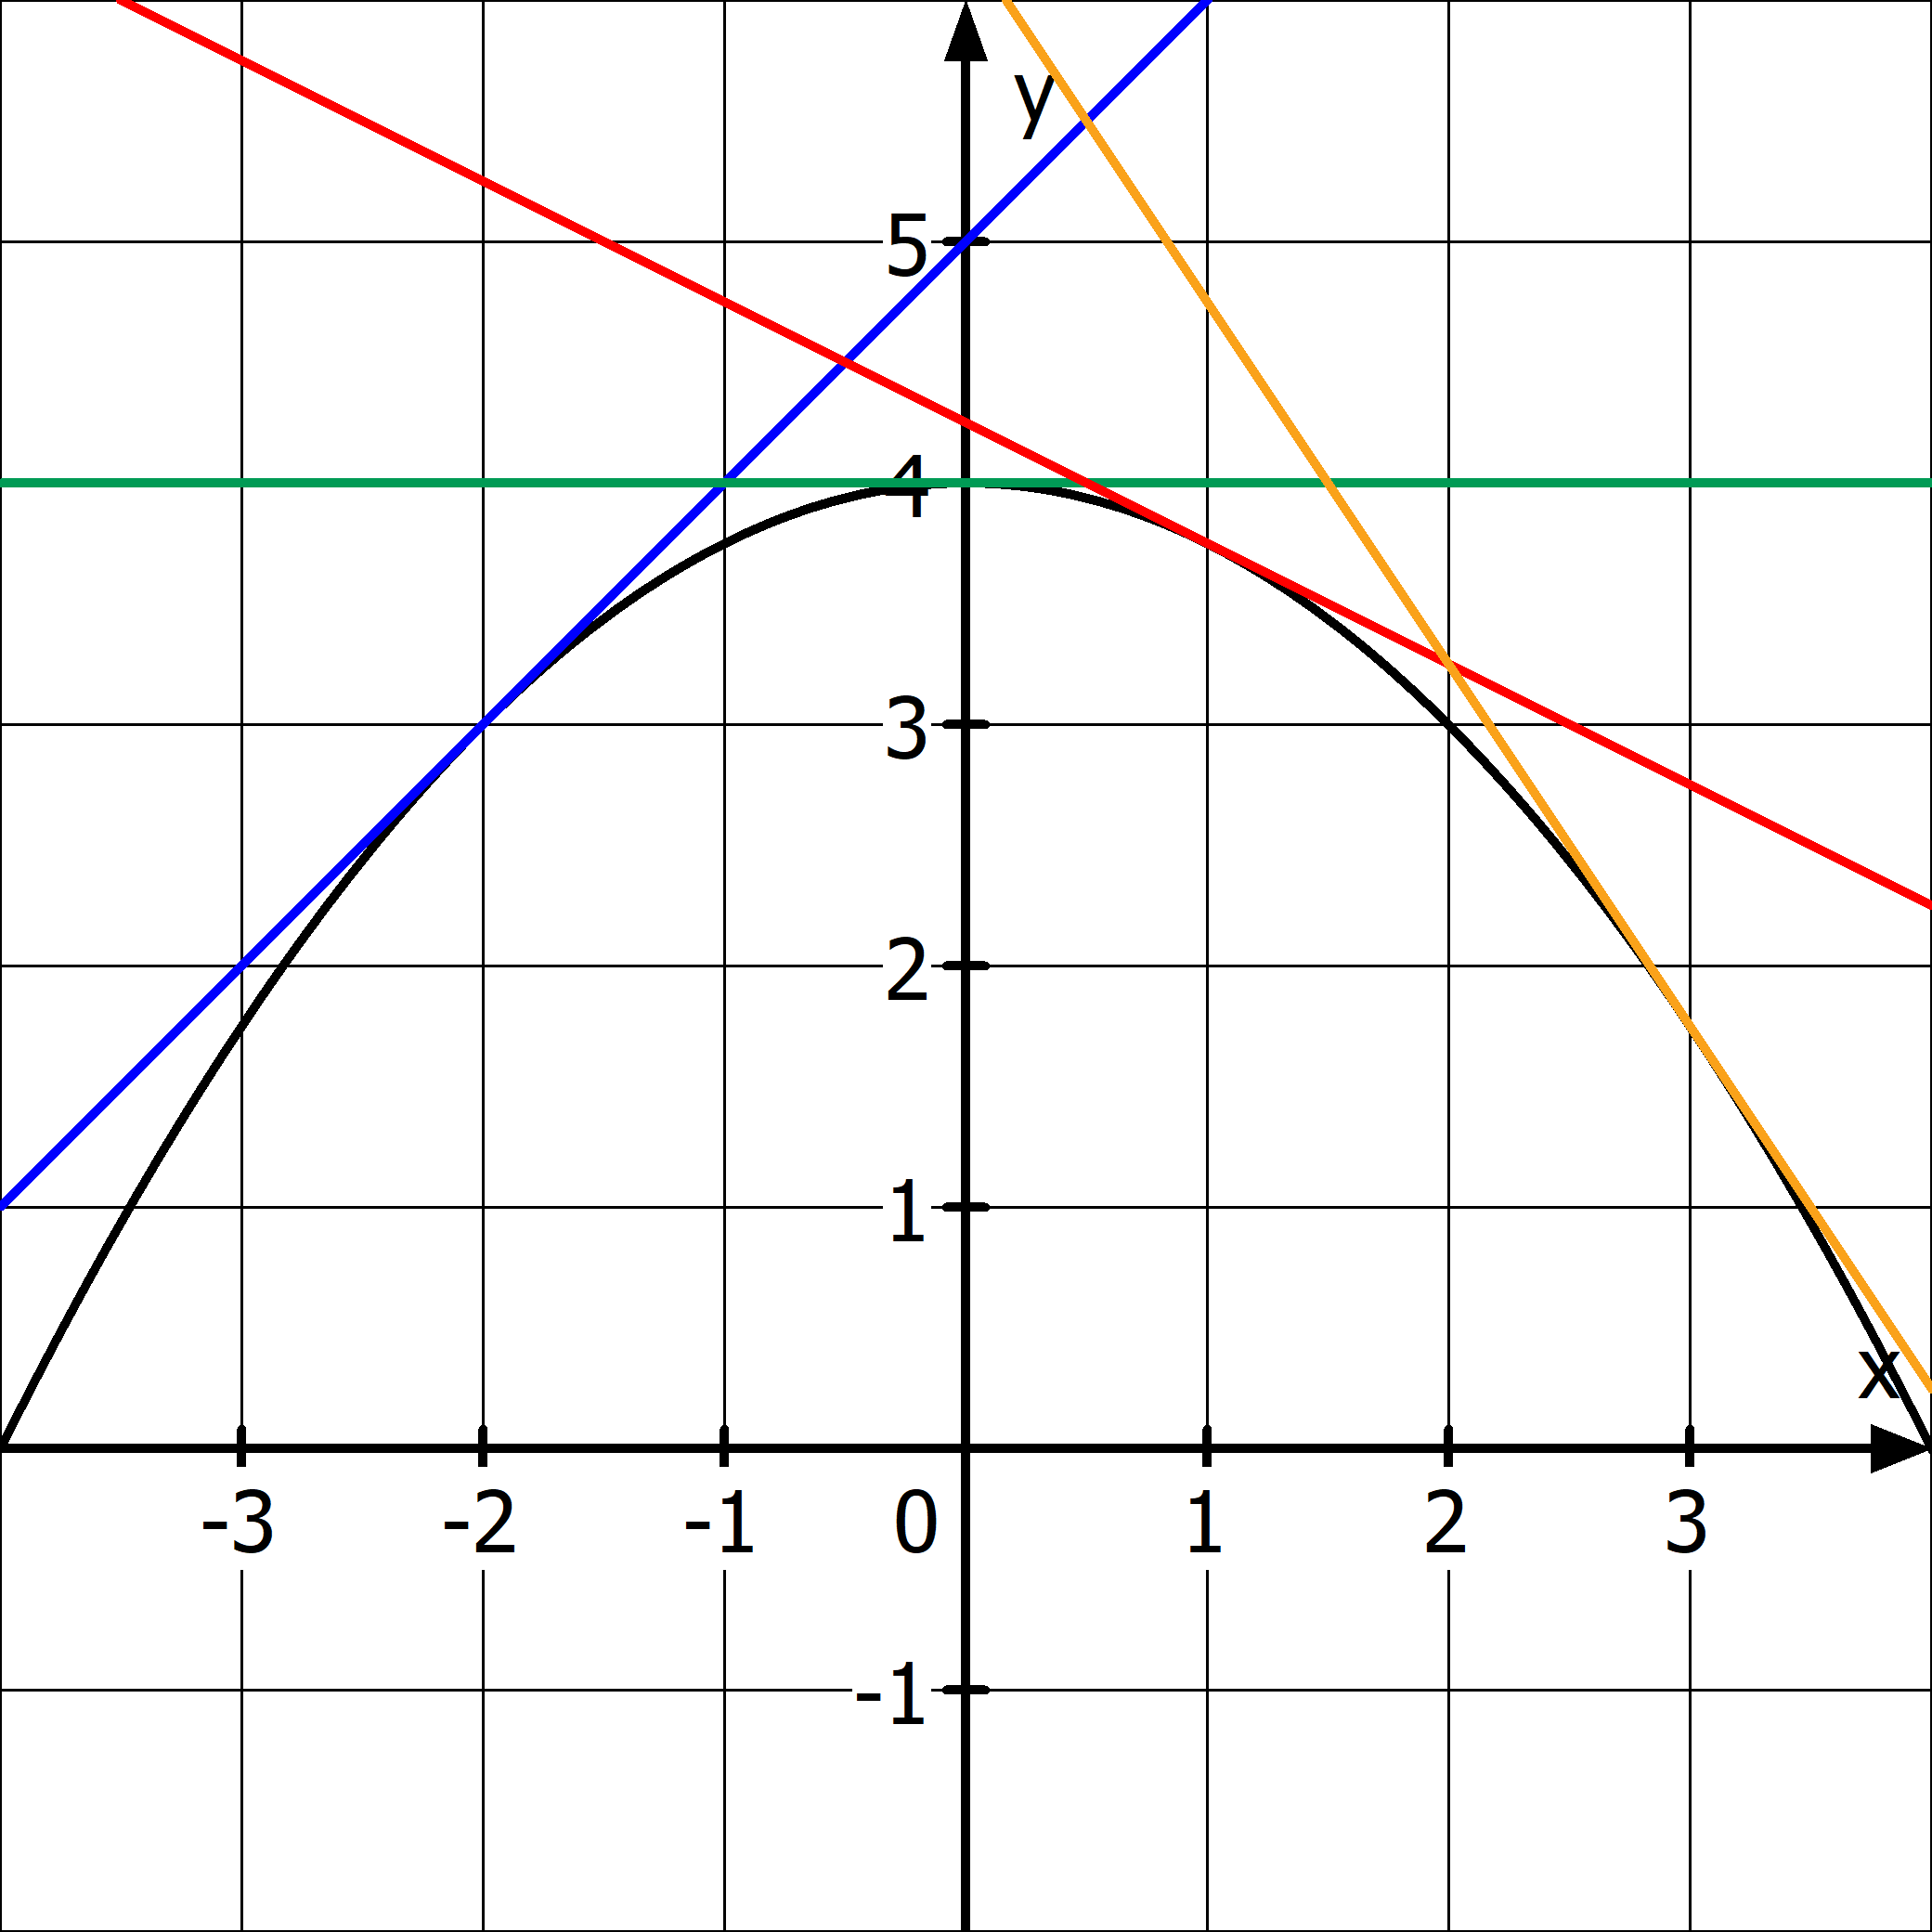
\includegraphics[width=.95\textwidth]{\ableitung/pics/grafisch2Loesung.png}\\
			\(\textcolor{blue}{f'(-2)\approx1}\)\\
			\(\textcolor{ForestGreen}{f'(0)\approx0}\)\\
			\(\textcolor{red}{f'(1)\approx-0,5}\)\\
			\(\textcolor{YellowOrange}{f'(3)\approx-1,5}\)\\
		\end{minipage}%
	\end{minipage}%


	\begin{minipage}{\textwidth}
		\begin{minipage}{0.5\textwidth}
			\centering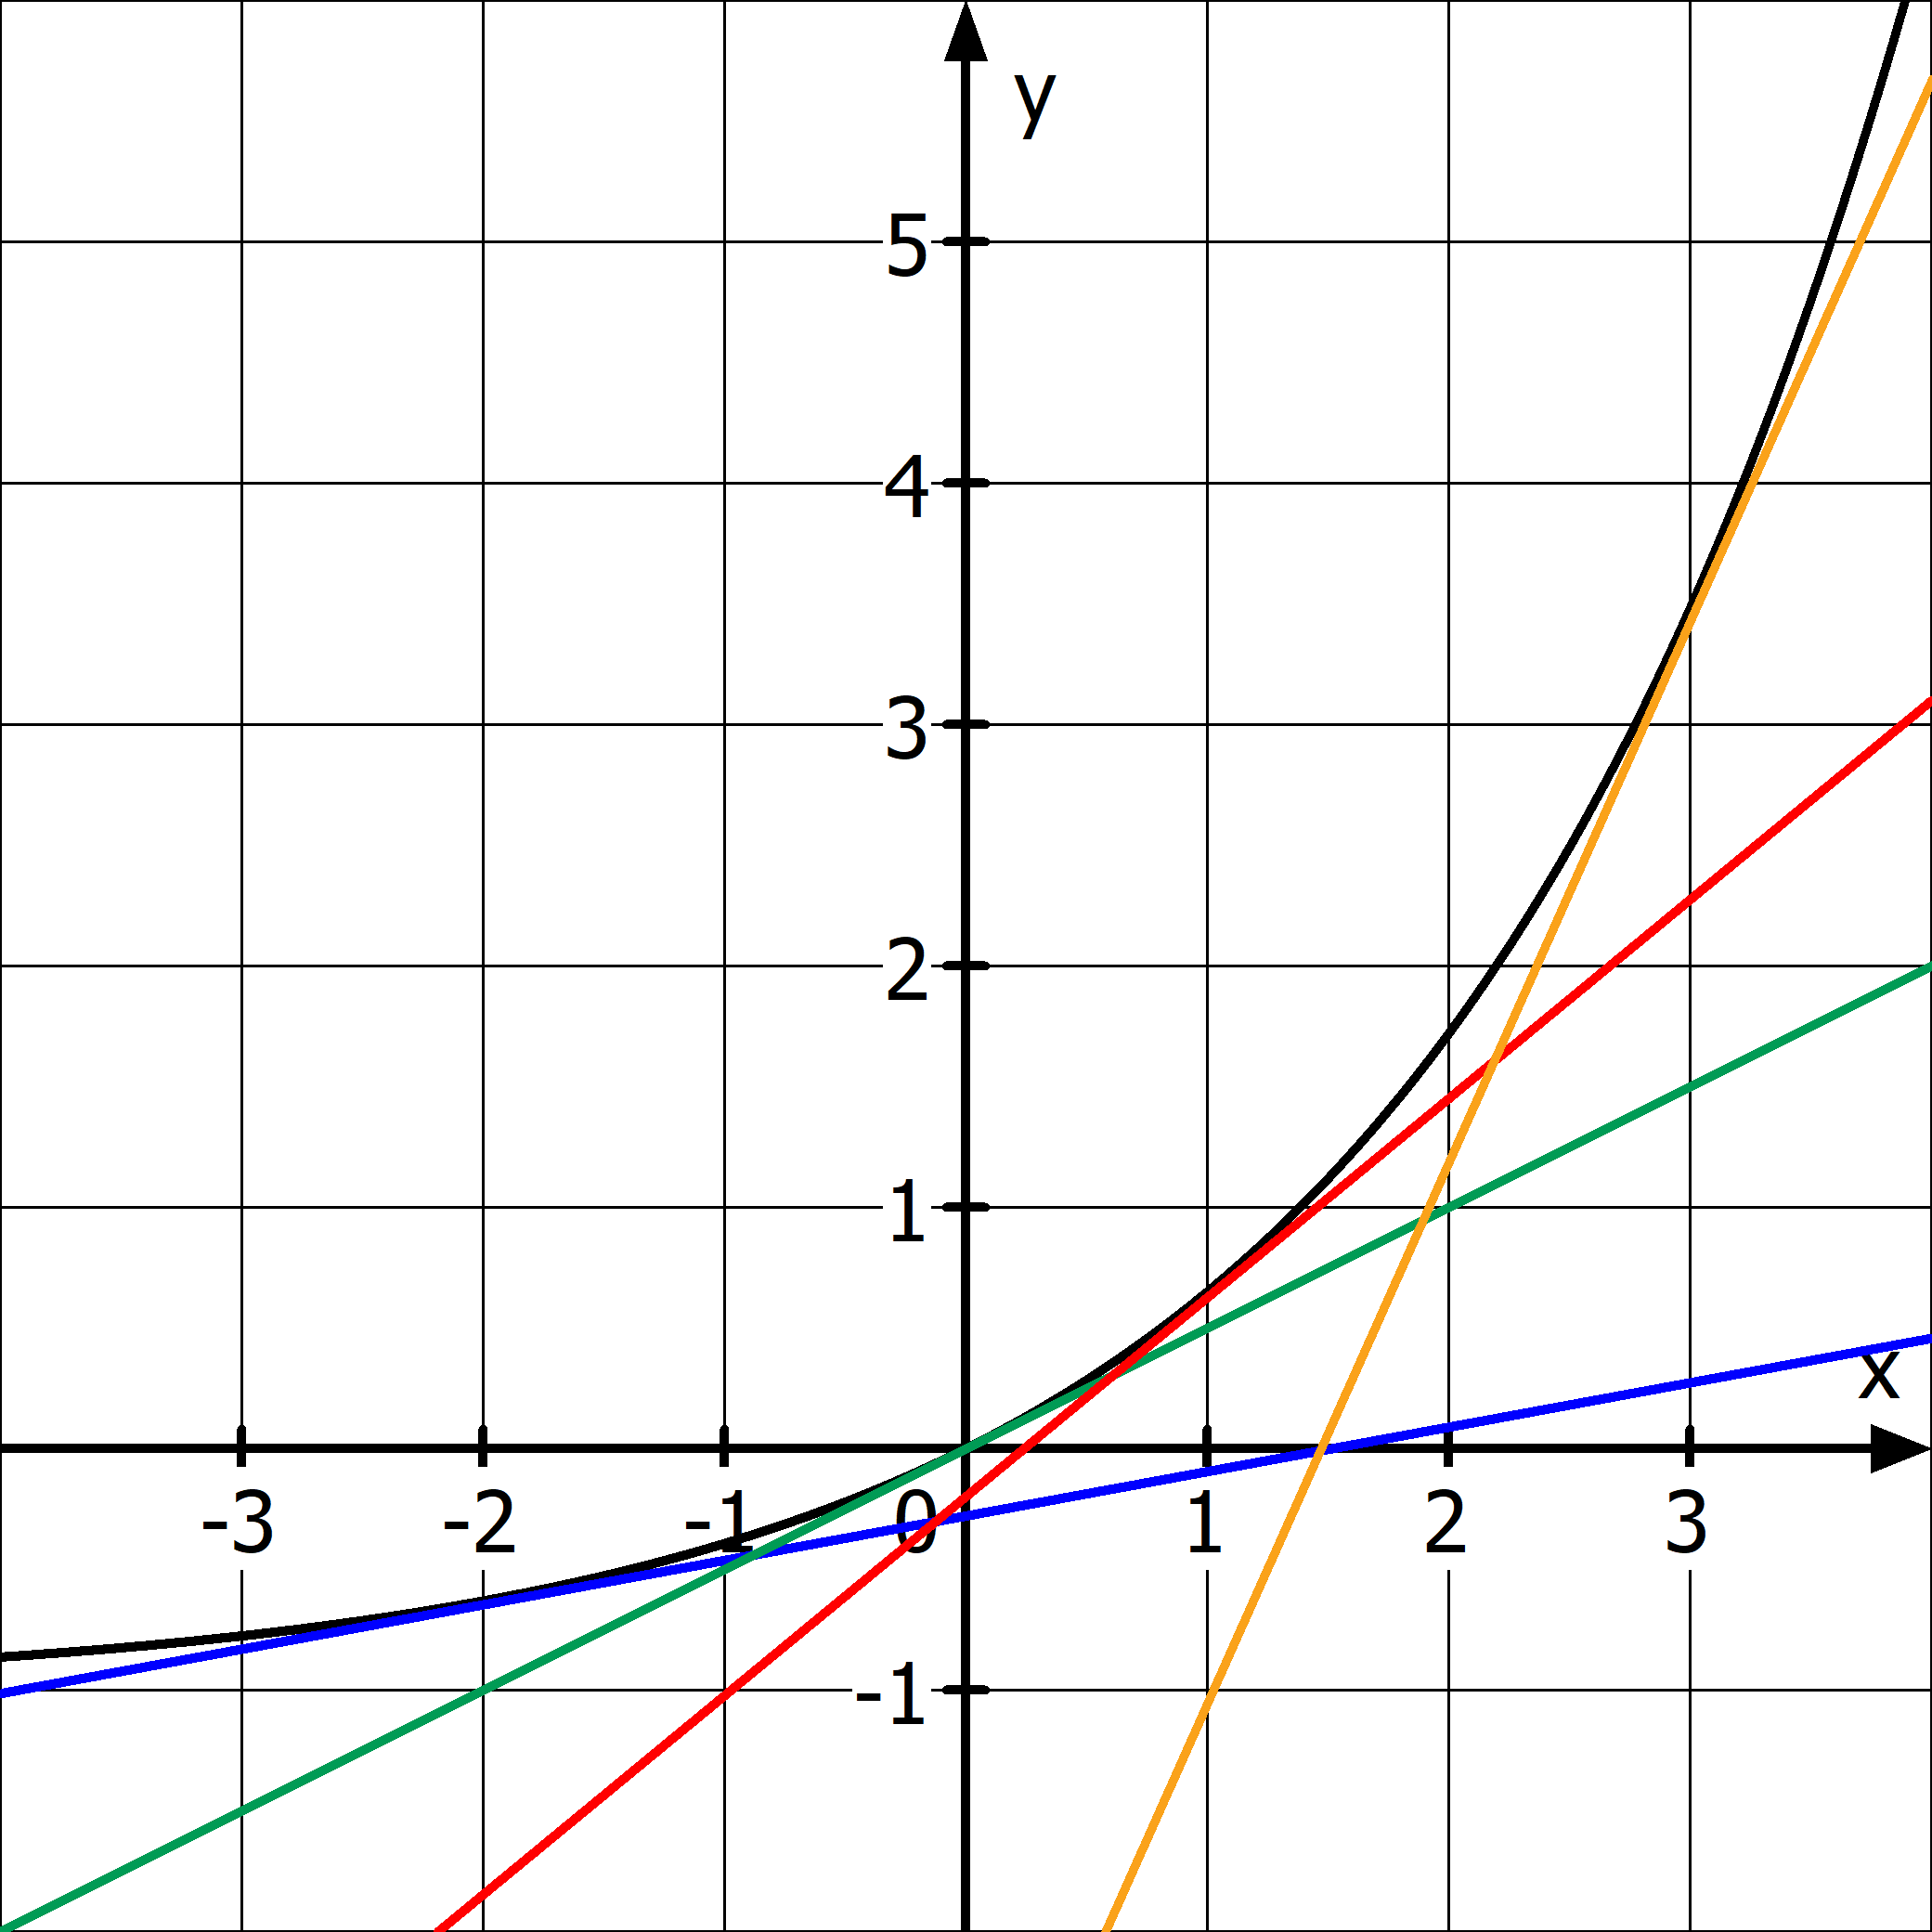
\includegraphics[width=.95\textwidth]{\ableitung/pics/grafisch3Loesung.png}\\
			\(\textcolor{blue}{f'(-2)\approx0,2}\)\\
			\(\textcolor{ForestGreen}{f'(0)\approx0,5}\)\\
			\(\textcolor{red}{f'(1)\approx0,8}\)\\
			\(\textcolor{YellowOrange}{f'(3)\approx2,25}\)\\
		\end{minipage}%
		\begin{minipage}{0.5\textwidth}
			\centering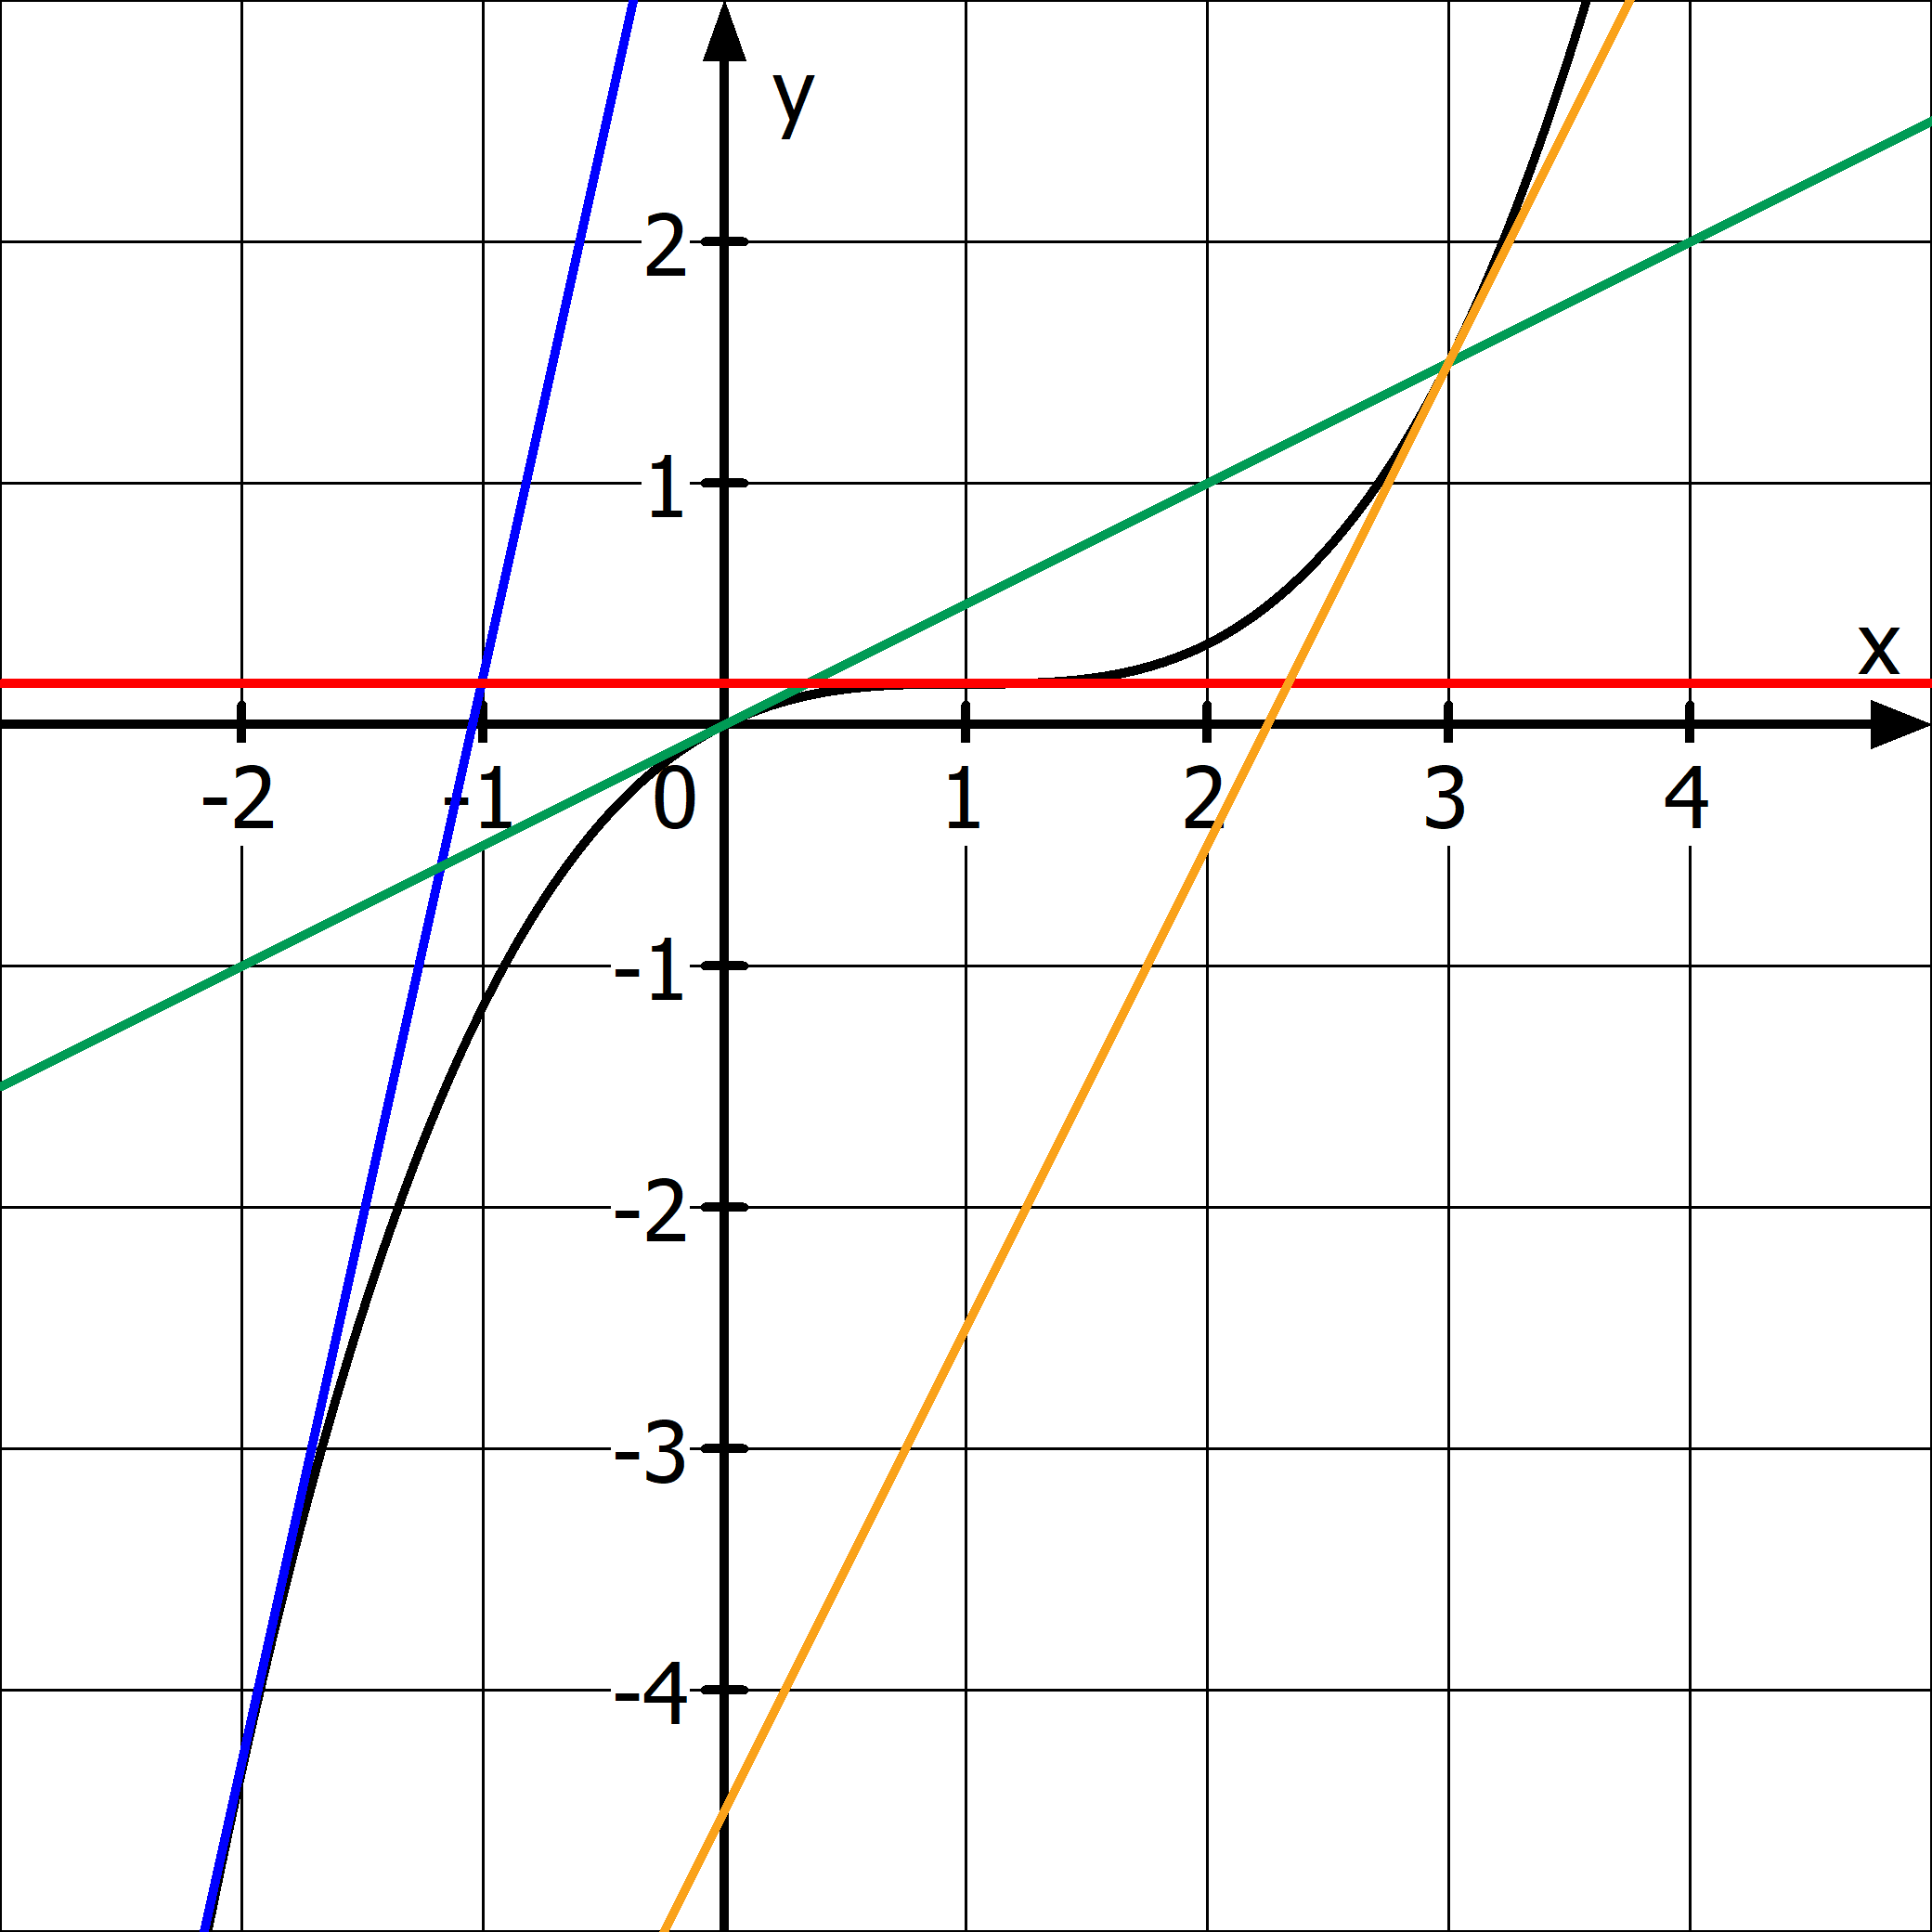
\includegraphics[width=.95\textwidth]{\ableitung/pics/grafisch4Loesung.png}\\
			\(\textcolor{blue}{f'(-2)\approx4,5}\)\\
			\(\textcolor{ForestGreen}{f'(0)\approx0,5}\)\\
			\(\textcolor{red}{f'(1)\approx0}\)\\
			\(\textcolor{YellowOrange}{f'(3)\approx2}\)\\
		\end{minipage}%
	\end{minipage}%
\end{Answer}